% \section*{Chapter 2}
% \addcontentsline{toc}{section}{Supporting Information Chapter 2}
\nobibliography* % suppresses bibliography at the end of the document

\urlstyle{same}
\begin{landscape}
\begin{table}[!ht]
\caption[Information on mutational variance estimates obtained from the literature.]{\textbf{Information on mutational variance estimates obtained from the literature.} We detail estimates that were included in the meta-analysis (A) and those that were disqualified (B, C). For each paper, we detail the source of the estimates of scaled mutational variance (mutational heritability, $h_M^2$ and, coefficient of mutational variance, $CV_M$) and associated error estimates\textsuperscript{\textdagger}. Studies (or individual estimates within studies) with scaled estimate (and error) required for the meta-analysis, but which were excluded on based on some additional data criteria are listed (and exclusion justified) in (B). In C, we list papers (estimates) that were excluded due to insufficient information to obtain standard error estimates for the scaled mutational parameters. NB: Some papers appear in (A) and (B) or (C). Only estimates identified in (A) were included in the meta-analysis. Estimates are available at:  \url{https://figshare.com/articles/dataset/MA_dserrata_wings_csv/14913051}.}
\label{tab:TabS1}
\scriptsize
\singlespacing
% \renewcommand{\arraystretch}{1.25}
\vspace{-1.5em}
\begin{tabular}{>{\hangindent=2em}p{4.7in}>{\vspace{0em}}p{4.7in}}
  \toprule
Reference & {\vspace{-1em}}Description of where estimates were obtained from \\ 
  \midrule
& \\[-1.5ex]
 \multicolumn{2}{c}{\textbf{\MakeUppercase{(A) Estimates used in the Meta-analysis}}}\\ 
& \\[-2ex]
\bibentry{Avil02} & $CV_M$ from Halligan and Keightley$^1$ Table 1.\\
\bibentry{Azev02} & Table 1 of paper with scale of mean corrected based on Figure 1.\\
\bibentry{Baer05} & $h^2_M$, $V_M$ and $CV_M$ estimates calculated from information in paper’s Table 1 and Supplementary Tables 3, 4 and 5. Error estimated by sampling\textsuperscript{\textdagger}. \\
\bibentry{Baer10a} & Table 2 of paper; $V_M$ reported as $I = \frac{V_M}{\bar{X}^2}$ and therefore $CV_M$ calculated as: $100\times\sqrt{I}$. Confidence intervals from bootstrapping where parameter constrained to be positive. \\
\bibentry{Caba02} & $CV_M$ calculated from in-text information, taking $V_B$ from ${\Delta}V=V_B$ / ($mean_c \times F_c$); where $F_c=203$ and $mean_c = 0.625$. Error estimated by sampling\textsuperscript{\textdagger}.\\
\bibentry{Char04} & $CV_M$ (and error) estimates taken from Halligan and Keightley$^1$ Table 1. \\
\bibentry{Clar95} & Trait means were taken from Table 1. $h^2_M$ and $V_M$ estimates taken from Table 4; $V_M$ was multiplied by 2.5 (scale for whole genome, as stated by authors) before calculating $CV_M$. Error in $CV_M$ estimated by sampling\textsuperscript{\textdagger}. \\
\bibentry{Davi16} & Table S1 of paper. Note: No estimate of $CV_M$ for citric acid as mean mis-reported in Table S1 and correct value unknown.  Confidence intervals from bootstrapping where parameter constrained to be positive. \\
\bibentry{Este05} & We calculated $CV_M$ using $V_M$ (Table 1) and the mean from Table 1 of the companion paper by Ajie \textit{et al.}$^3$. $h2_M$ was from Table 1 of Ajie \textit{et al.}$^3$  \\
\bibentry{Etie15} & Table 1 of paper.  Error in $h^2_M$ estimated by sampling\textsuperscript{\textdagger}.  Confidence intervals from bootstrapping where parameter constrained to be positive. \\
% ========Gap =======&
\bottomrule
\end{tabular}
\end{table}
\begin{table}[!ht]
\vspace{-0.5em}
\scriptsize
\singlespacing
\renewcommand{\arraystretch}{0.9}
\begin{tabular}{>{\hangindent=2em}p{4.7in}>{\vspace{0em}}p{4.7in}}
\midrule
% ========Gap =======&
\bibentry{Fern96} & $V_M$ and $h^2_M$ taken from Table 3 and trait mean from Table 1 of paper; $CV_M$ calculated from those estimates (but no error estimate available). \\
\bibentry{Fry02} & Trait means were from Table 1 and mutational variances were from Table 3; $CV_M$ was calculated from those estimates. Error estimated by sampling\textsuperscript{\textdagger}.  \\
\bibentry{Fry99} & Trait means and mutational variances were from Fry and Heinsohn (2002)’s Table 1 and Table 3, respectively, where $CV_M$ was calculated from those estimates.  \\
\bibentry{Garc00} & Table 2 of paper. \\
\bibentry{Hara95} & $CV_M$ was calculated from information in Table 3 and 4 of paper; $V_M$ was calculated using $4V_G$ (reported) and divided by $2\times$ the number of generations. Error estimated by sampling\textsuperscript{\textdagger}.  \\
\bibentry{Houl94} & $V_M$ from Table 4 of paper ($\times 2.5$ to scale to genomewide as indicated by the authors); data was standardised to mean=1 prior to estimation, and $CV_M = 100*\sqrt{V_M}$. Error estimated by sampling\textsuperscript{\textdagger}. \\
\bibentry{Houl04} & Table 3 of paper (for IVe-39 sublines only, constrained intercept), where $CV_M = 100*\sqrt{\Delta{V}}$ as described in text of paper on page 9. Error estimated by sampling\textsuperscript{\textdagger}. \\
\bibentry{Joyn09} & Table 1 and 2 of paper.\\
\bibentry{Keig97} & $h^2_M$ estimate (and SE) provided in text on pg 3825. Estimates for productivity determined from among-line variances and trait mean taken from Figure 2 using the R package \textit{metaDigitise}. Error in $CV_M$ estimated by sampling\textsuperscript{\textdagger}. \\
\bibentry{Lati14} & Table 1 of paper \\
\bibentry{Lope93} & We used estimates from B (full-sib mating) lines only, where trait means were from figure 1 (males=30, females = 36.8). Among-line variance and $h^2_M$ for bristle number from Table 6, $CV_M$ calculated from the provided information, but no error estimate available.\\
\bibentry{Lync85} & $h^2_M$ from Table 1 and $CV_M$ calculated from information in Table 1 (but no SE provided for mean and hence unavailable for $CV_M$). Error estimated by sampling\textsuperscript{\textdagger}.\\
\bibentry{Lync98b} & Estimates of $h^2_M$, $V_M$, $V_E$ and trait mean (MA mean calculated for the final generation as: $z_0+R_m*30$) from Table 1 of paper and $CV_M$ calculated from this information. Error in $CV_M$ estimated by sampling\textsuperscript{\textdagger}: $z_0$ and $R_m$ were sampled to allow the mean to be determined per sample.\\
\bibentry{Mack92B} & Table 3 of paper, assuming $N = 0.7N_e$. Estimates available for per generation (Table 1), but SE not reported.\\
\bibentry{Mart98} & Table 2 of paper. \\
\bibentry{McGu11a} & $h^2_M$ was taken from text. $CV_M$ was calculated by determining $V_M$ as (mean ($V_E$) × $h^2_M$), where $V_E$ and MA means were taken from Tables S1 and S2 of paper for the Control MA population. Error estimated by sampling\textsuperscript{\textdagger}.\\
% ========Gap =======&
\bottomrule
\end{tabular}
\end{table}
\begin{table}[!ht]
\vspace{-0.em}
\scriptsize
\singlespacing
\renewcommand{\arraystretch}{0.95}
\begin{tabular}{>{\hangindent=2em}p{4.7in}>{\vspace{0em}}p{4.7in}}
\midrule
% ========Gap =======&
\bibentry{Muka72} & Among-line and mean estimates from Tables 1, 2 and 3 of paper for Generation 40 only were used to calculate $V_M$ and $CV_M$.\\
\bibentry{Ostr07} & Trait mean from Table 1 and $CV_M$ (MA mean), $V_M$ and $h^2_M$ from Table 2 of paper. While log transformation had little impact on scaled estimates, $V_M$ and $V_E$ were extreme on the raw scale, while mean of the log-transformed data was negative.\\
\bibentry{Plet98} & $h^2_M$, $V_M$ and mean from Table 5 of paper and $CV_M$ estimated from that information. Error estimated by sampling\textsuperscript{\textdagger}.\\
\bibentry{Role16} & Table 2 of paper. We included $CV_M$ for fruit number and total fitness however authors have calculated $CV_M$ as $100(e^{\sqrt{V_M}}-1)$ as per Poisson values. Parameter confidence intervals from MCMCglmm, and constrained to be positive. \\
\bibentry{Rutt10} & Table 2 of paper. \\
\bibentry{Sant92} & $h^2_M$ and $V_E$ from Table 4 for full-sib mating lines only (B lines; all lines). Trait means were taken from Figure 3 (sternopleural bristles =21.7, wing length = 1210 and wing width = 465). $CV_M$ estimated from that information but error estimates not available.\\
\bibentry{Scho05} & Trait means and mutational variances were taken from Table 1 and 3 for flower number and weight
respectively. $V_M$, $h^2_M$, and $CV_M$ were estimated from that information, where $V_L$ for MA was corrected for
initial (control variance) if that was non-zero; error estimates were similar between control and mutant and
MA SE were used to approximate error for meta-analysis.\\
\bibentry{Schu99} & From Table 3; $CV_M$ not available as calculated from among-line variance, not the per-generation $V_M$.\\
\bibentry{Shaw00} & Estimates of mean and among-line and environmental variances taken from Table 1 of paper (generation 17), and estimates of $V_M$, $h^2_M$, and $CV_M$ from Table 2. To estimate error for $h^2_M$, and $CV_M$, the among-line and mean estimates for generation 17 were used, along with $V_M$ from the joint analysis. Error estimated by sampling\textsuperscript{\textdagger}.\\
\bibentry{Vass00} & $h^2_M$ was taken from Table 2; trait mean (intercept) from Table 1 and $V_M$ ($slope/2$) from Table 2 were used to calculate $CV_M$. Error in $CV_M$ estimated by sampling\textsuperscript{\textdagger} following the approach detailed for Lynch \textit{et al.} (1998) above. For one trait (generation time) the reported standard error of the $V_M$ was 0, precluding calculation of errors. \\
\bibentry{Vass99} & $h^2_M$ and $V_M$ estimates were taken from Table 1 of paper. Error in $CV_M$ estimated by sampling\textsuperscript{\textdagger} following the approach detailed for Lynch \textit{et al.} (1998) above. For one trait (generation time) the estimated mean was $\sim0$, resulting in nonsensical $CV_M$ and hence this was excluded.\\
  \midrule
& \\[-1.5ex]
 \multicolumn{2}{c}{\textbf{\MakeUppercase{(B) ESTIMATES REMOVED FROM META-ANALYSIS DUE TO ISSUES WITH MUTATIONAL PARAMETER ESTIMATES}}}\\ 
& \\[-2ex]
\bibentry{Baer10a} & As in (A); Excluded \textit{Caenorhabditis brenneri} strain PB2801 $h^2_M$ and strain PB2802 $CV_M$ generation 100 estimates as they were outliers ($>3.5$ standard deviations from the mean and $>5$ times the inter-quartile range from the median).\\
\bibentry{Bail59} & From Table 1, and in-text information on number of generations; $h^2_m$ calculated as per Lynch $1988^4$. Excluded due to low representation of vertebrate taxa.\\
% ========Gap =======&
\bottomrule
\end{tabular}
\end{table}
\begin{table}[!ht]
\vspace{-0.5em}
\scriptsize
\singlespacing
% \renewcommand{\arraystretch}{1.25}
\begin{tabular}{>{\hangindent=2em}p{4.7in}>{\vspace{0em}}p{4.7in}}
\midrule
% ========Gap =======&
\bibentry{Case08} & MA litter mean was taken for generation 46 in Table 1. The $V_M$ and $h^2_m$ estimates were taken from text and Table 3. $CV_M$ was calculated from reported information. Excluded due to low representation of vertebrate taxa.\\
\bibentry{Clar95} & As in (A). ADH $h^2_m$ excluded as it was an extreme outlier ($>4$ standard deviations from the mean and $>5$ times the inter-quartile range from the median).\\
\bibentry{Down03} & $V_M$ and $h^2_m$ were taken from Table 1. Line means were estimated from figure 3 and used to calculate $CV_M$ (but not error). Excluded due to low representation of non-Drosophila insect taxa.\\
\bibentry{Farh16} & Trait means from Table 1 of paper, and variances from Table S4. One estimate (for posterior centrosome oscillation frequency) was removed as the estimate for $V_M$ was negative. Excluded due to low representation of trait type (mitotic cell division).\\
\bibentry{Hara95} & As in (A); Could not calculate $CV_M$ (negative mean) for one metabolite (Isocitrate-dehydrogenase activity) which was therefore excluded. Alpha-amalyse was excluded as the estimated SE of $CV_M$ was considerably larger than the estimate itself.\\
\bibentry{Houl94} & As in (A). Early male mating success excluded as $CV_M$ estimate was negative; late mating $CV_M$ excluded due extreme value ($>4$ standard deviations from the mean and $>5$ times the inter-quartile range from the median)\\
\bibentry{Joyn11} & Information in Table 1 of paper used to calculate $CV_M = 100*\sqrt{V_M}$, where $V_M$ (and $V_L$) were reported on intensity of selection scale, as described on pg 1441 of paper. We sampled from the distribution of parameters used to calculate $V_M$, but the standard error of the sample was orders of magnitude larger than the estimate. Therefore, this study was excluded.\\
\bibentry{Latt15} & Among-line variance (designated by authors as $\Delta$V) provided in Table S1 and used to calculated using $V_M = \Delta$V/(2*96), where 96 was the number of generations of MA reported by the authors on pg 245 of paper. $V_E$ and $\bar{X}$ were provided in Table S1 and, along with the calculated $V_M$, used to calculate $h^2_m$ and $CV_M$. However, the
reported confidence intervals for $\Delta$V are extremely large (infinite for several traits), and the standard errors calculated are always larger than the parameter estimate, and all estimates from this study were excluded. Notably, this study included only five MA lines, and poor quality estimates could be expected.\\
\bibentry{Lope93} & \\
\bibentry{Lync98} & As in (A). Second clutch size excluded as it was an extreme outlier ($>7$ standard deviations from the mean and $>5$ times the inter-quartile range from the median). Size at birth was excluded because calculation of $h^2_m$ from the data in Table 1 returned an estimate several orders of magnitude larger than reported, suggesting some incorrect parameter values reported. \\
\bibentry{Morg14} & $CV_M$ estimates were taken from Table 3 (second assay only, as one strain had missing data for the first assay), but no SE reported. To estimate SE it was necessary to use $V_L$ estimates for MA and ancestor from Table 3 (and reported CI), the generation number estimates from Table 2, and estimates of trait mean (CI) from Table 4. Excluded due to low representation of micro-organisms.\\
\bibentry{Pann08} & MA mean and line numbers taken from Table 2 of paper. Variance estimates were taken from Table 3, where $CV_M$ has been converted to a percentage scale. Excluded due to low representation of non-Drosophila insect taxa\\
% ========Gap =======&
\bottomrule
\end{tabular}
\end{table}
\begin{table}[!ht]
\vspace{-0.5em}
\scriptsize
\singlespacing
% \renewcommand{\arraystretch}{1.25}
\begin{tabular}{>{\hangindent=2em}p{4.7in}>{\vspace{0em}}p{4.7in}}
\midrule
% ========Gap =======&
  % \midrule
& \\[-1.5ex]
 \multicolumn{2}{c}{\textbf{\MakeUppercase{(C) ESTIMATES REMOVED FROM META-ANALYSIS DUE TO LACK OF INFORMATION ON ESTIMATION ERROR OF A MUTATIONAL PARAMETER}}}\\ 
& \\[-2ex]
\bibentry{Burc07} & $V_M$ was calculated from the log fitness variances reported on pg. 473, and MA mean was calculated as $1 - E(log W_1)$ to calculate $CV_M$.\\
\bibentry{Chan03} & Table 3 of paper.\\
\bibentry{Clar93} & Halligan \& Keightley$^1$ Table 1; no further detail in original paper to estimate SE.\\
\bibentry{Fest73} & Houle \textit{et al.} (1996)$^2$ Table 1; insufficient information in the original paper to determine error for scaled variance
estimates. \\
\bibentry{Gong05} & $CV_M$ estimates were taken from Halligan \& Keightley$^1$ Table 1, but were noted by. Halligan \& Keightley$^1$ as extreme outliers. Insufficient information to calculate errors for scaled estimates.\\
\bibentry{Hall08} & Table 2 of paper.\\
\bibentry{Huan16} & $h^2_m$ estimates were taken from supplementary information 1D but no estimate of error provided. \\
\bibentry{Jose04} & From in-text information on page 1819; NB: heritability estimate was incorrectly reported and corrected in Hall \textit{et al.} 2008 (citation details above) \\
\bibentry{Kava05} & Estimates from information in Table 5 of paper, but no errors reported in that table. Notably several estimates of mutational variance were negative (Table 5), and mutational variance was not statistically supported for any trait in this study.\\
\bibentry{Keig97} & Lifespan estimates were taken from text on p. 3826 of paper but no error estimate reported.\\
\bibentry{Kibo96} & Halligan \& Keightley$^1$ Table 1; no further detail in original paper to estimate SE.\\
\bibentry{Mack98} & Table 9 of paper: Only the MA maintenance temperature was recorded. No error estimates.\\
\bibentry{Muka64} & Houle \textit{et al.} (1996)$^2$ Table 1; $V_E$ complexity detailed in Houle \textit{et al.} (1996)$^2$ and lack of information on mean
error mean that no SE of scaled $V_M$ were obtained.\\
\bibentry{Muka68} & Table 1 of paper; no further detail in original paper to estimate SE of scaled $V_M$. \\
\bibentry{Muka84} & Table 1 and in text. Insufficient information to obtain error estimate for scaled estimate of $V_M$.\\
\bibentry{Ohni77} & Table 1 and in text (for zero level of mutagen only), but insufficient information to calculate SE for scaled estimates; Houle \textit{et al.} (1996)$^2$ Table 1.\\
% ========Gap =======&
\bottomrule
\end{tabular}
\end{table}
\begin{table}[!ht]
\vspace{-0.5em}
\scriptsize
\singlespacing
% \renewcommand{\arraystretch}{1.25}
\begin{tabular}{>{\hangindent=2em}p{4.7in}>{\vspace{0em}}p{4.7in}}
\midrule
% ========Gap =======&
\bibentry{Paxm57} & Houle \textit{et al.} (1996)$^2$ Table 1; no further detail in original paper to estimate SE.\\
\bibentry{Plet99} & Estimates of $V_M$ from Table 4 of paper, but no estimates of error of trait mean or $V_E$ reported and no scaled estimate with associated error derived. \\
\bibentry{Russ63} & Houle \textit{et al.} (1996)$^2$ Table 1; no further detail in original paper to estimate SE. The authors note (pp 177) that their genetic variation are “rather poorly estimated”. \\
\bibentry{Wayn98} & Table 3 of paper.\\
\bibentry{Xu04} & $h^2_m$ estimates from Table 2 of paper.\\
% ========Gap =======&
\bottomrule
\end{tabular}
\end{table}
\begin{table}[!ht]
\vspace{-19cm}
\tiny
\singlespacing
\renewcommand{\arraystretch}{2}
\begin{tabular}l
\textsuperscript{\textdagger} Where 95\% confidence intervals were reported, we converted to approximate standard errors as: (upper limit – lower limit) / 3.92. Where standard errors were not reported for $h^2_M$ or $CV_M$, but were reported for the parameters used to calculate these scaled mutational variance \\[-1em]
estimates (e.g., $V_M$, $V_E$, mean), as described in the Methods, we used the `rnorm` function in R to generate 10,000 random samples from the distribution defined by the estimate (mean) and standard error (variance), and calculated the scaled metric (for $h^2_M$ or $CV_M$) in each \\[-1em]
sample, then estimated the standard error.\\
$^1$ \bibentry{Hall09} \\
$^2$ \bibentry{Houl96}\\
$^3$ \bibentry{Ajie05} \\
$^4$ \bibentry{Lync88b} \\
% ========Gap =======&
\end{tabular}
\end{table}
\end{landscape}
\nobibliography{}
% \nobibliography{DFElib}

 



\newpage
\begin{table}[!ht]
    \caption[Trait types included in the broad categories and within the more narrowly defined life history trait categories.]{\textbf{Trait types included in the broad categories and within the more narrowly defined life history trait categories.} The trait description is a list of traits included within each category.}
    \centering
    \small
    \renewcommand{\arraystretch}{1.45}
    \begin{tabular}{>{\centering\arraybackslash}p{2cm}>{\centering\arraybackslash}p{2.8cm}>{\centering\arraybackslash}p{10.2cm}}
    \toprule
         {\centering Broad \\ Category} & {\centering Narrow \\ Category} & Trait Description\\
    \midrule
Life-history & 
Fitness & Fitness; Intrinsic rate of increase; Competitive mating success; Rate of convergence to the stable age distribution. \\
& Miscellaneous & Longevity, Lifespan, Male mating success, Age at maturity, Age at reproduction,Growth rate, Instar duration, The reciprocal of the mean age at reproduction, Time to maturity.\\
    & Productivity & Clutch size, Fecundity, Litter size, Number of flowers, Seed count, Productivity,
Reproductive mass\\
    & Survival & Survival, Age-specific survivorship or viability,  Germination, Pathogen susceptibility.\\
Morphology & - & Abdominal and sternopleural bristles; Body length, width or size; Limb/Organ/Spine length or width, Weight.\\
Physiology & - &  Enzyme activity, Metabolites, Locomotor activity, Velocity.\\
    \bottomrule
    \end{tabular}
    \label{tab:TraitTypes}
\end{table}

\newpage
\begin{table}[!h]
    \centering
    \renewcommand{\arraystretch}{1.3}
    \scriptsize
        \caption[Mutation accumulation (MA) lines shared across studies.]{\textbf{Mutation accumulation (MA) lines shared across studies.} The first published description of a set of MA lines is indicated in bold; the following non-bolded entries represent subsequent investigations of the same set of MA lines. See Table \ref{tab:TabS1} for citation details.}
    \begin{tabular}{llcl}
    \toprule
    Species name & Reference & Generation & Trait Description\\
    \midrule
\textit{Arabidopsis thaliana }
    & \textbf{Shaw \textit{et al.} (2000)} & 17 & Fecundity, Reproductive mass\\
    & Rutter \textit{et al.} (2010) & 25 & Fecundity \\
    & Roles \textit{et al.} (2016) & 25 & Fecundity, Germination, Age-specific survivorship, Fitness\\
    \midrule
\textit{Caenorhabditis briggsae} 
    & \textbf{Baer \textit{et al.} (2005)} & 200 & Productivity\\
    & Ostrow \textit{et al.} (2007) & 200 & Body size\\
    & Joyner-Matos \textit{et al.} (2009) & 250 & Life span\\
    \midrule
\textit{Caenorhabditis elegans}
    & \textbf{Baer \textit{et al.} (2005)} & 200 & Productivity\\
    & Ostrow \textit{et al.} (2007) & 200 & Body size\\
    & Joyner-Matos \textit{et al.} (2009) & 250 & Life span\\
    & Etienne \textit{et al.} (2015) & 250 & Pathogen susceptibility\\
    & Davies \textit{et al.} (2016) & 250 & Metabolites\\
    & \textbf{Keightley \& Caballero (1997)} & 60 & Lifespan, Productivity, Population growth\\
    & Azevedo \textit{et al.} (2002) & 60 & Body size\\
    & \textbf{Vassilieva \textit{et al.} (1999)} & 49.4 & Longevity, Productivity, Survivorship, Population growth\\
    & Vassilieva \textit{et al.} (2000) & 214 & Longevity, Productivity, Survivorship, Population growth\\
    & Azevedo \textit{et al.} (2002) & 152 & Body size\\
    & Estes \textit{et al.} and Ajie \textit{et al.} (2005) & 370 & Population growth parameter, Body width Locomotor activity, \\
    & & & Productivity, Velocity\\
    \midrule
\textit{Drosophila melanogaster }
    & \textbf{Houle \textit{et al.} (1994)} & 44 & Fecundity, Fitness, Longevity, Male mating, Productivity\\
    & Pletcher \textit{et al.} (1998) & 19 & Female longevity, Male longevity\\
    & \textbf{Santiago \textit{et al.} (1992)} & 46 & Sternopleural bristles, Wing dimensions\\
    & Fernandez \& Lopez-Fanjul (1996) & 106 & Viability, Fecundity \\
    & Martorell \textit{et al.} (1998) & 82 & Productivity, Longevity\\
    & Garcia-Dorado \textit{et al.} (2000) & 170 & Wing length\\
        & & 204 & Abdominal bristles, Sternopleural bristle\\
        & & 209 & Viability\\
    & Caballero \textit{et al.} (2002) & 210 & Viability\\
    & Avila \& Garca-Dorado (2002) & 288 & Fitness\\
    \midrule
\textit{Drosophila serrata }
    & \textbf{McGuigan \textit{et al.} (2011)} & 23 & Mating Success\\
    & & 26 & Productivity\\
    & Latimer \textit{et al.} (2014) & 32 & Locomotor activity \\
    \midrule
\textit{Oscheius myriophila }
    & \textbf{Baer \textit{et al.} (2005)} & 200 & Productivity \\
    & Ostrow \textit{et al.} (2007) & 200 & Body size \\
    \bottomrule
    \end{tabular}
    \label{tab:MetaNonIndepend}
\end{table}

\newpage
\FloatBarrier
\begin{landscape}
\begin{table}[!ht]
    \setlength\tabcolsep{0.3em}
    \tiny
    \caption[Parameter estimates from analyses of data for each of the 11 traits in each generation for each treatment in the \textit{Drosophila serrata} experiment.]{\textbf{Parameter estimates from analyses of data for each of the 11 traits in each generation for each treatment in the \textit{Drosophila serrata} experiment.} Model (\ref{eqn:metaUniVL}) was fit to data for each trait in each generation for each population size treatment. The least squares trait mean was estimated, and the phenotypic variance was partitioned to among-line (due to mutation), among the two replicate rearing vials nested within each line, and to the residual (among individuals within each vial) variances. We estimated the environmental variance as the sum of among-vial and among-individual (residual) variances. We placed the estimates of among-line variance on both a heritability (among-line variance / environmental variance) and coefficient of variance ($100* \sqrt{}$Among-line / Mean) scales but note that these should not be interpreted as mutational heritability or coefficient of variance because they are calculated from the total accumulated mutational variance (among-line variance) not the per generation rate at which that accrued. For each parameter, confidence intervals were estimated by drawing 10,000 random samples from a normal distribution with a mean equal to the REML model estimate and variance equal to either the inverse of the Fisher information matrix (for variance parameters) or the standard deviation (for the trait mean), as described in the Methods. From the 10,000 samples, 95\% (Mean) or 90\% (all other parameters, which are constrained to be positive) confidence intervals (CI) are reported. The environmental variance, heritability and coefficient of variance) were calculated for each of the 10,000 samples to estimate the CI of these calculated parameters. Statistical support for non-zero estimates was inferred where the lower CI did not include zero. Where REML parameter estimates were zero, no CI were estimated. }
    \label{tab:S4RegCoef}
        \centering
    \begin{tabular}{cccrlrlrlrlrlrlrl}
    \toprule
    	&&&	\multicolumn{2}{c}{Mean} & \multicolumn{2}{c}{Among-Line Variance ($\times10^4$)}&	\multicolumn{2}{c}{Among-Vial Variance ($\times10^4$)}& \multicolumn{2}{c}{Among-Individual Variance ($\times10^4$)} & \multicolumn{2}{c}{Environmental Variance ($\times10^4$)} & \multicolumn{2}{c}{Heritability} & \multicolumn{2}{c}{Coefficient of Variance}\\
    	\midrule
        Trait	&	Generation	&	Treatment	&	Estimate	&	\multicolumn{1}{c}{CI}	&	Estimate	&	\multicolumn{1}{c}{CI}	&	Estimate	&	\multicolumn{1}{c}{CI}	&	Estimate	&	\multicolumn{1}{c}{CI}	&	Estimate	&	\multicolumn{1}{c}{CI}	&	Estimate	&	\multicolumn{1}{c}{CI}	&	Estimate	&	\multicolumn{1}{c}{CI}	\\
        \midrule
        Size	&	1	&	Small	&	1.5533	&	(1.5479, 1.5590)	&	1.22	&	(-0.1893, 2.6234)	&	2.86	&	(1.3896, 4.3164)	&	4.74	&	(4.1377, 5.3282)	&	7.6	&	(6.0591, 9.1344)	&	0.1605	&	(-0.0225, 0.3952)	&	0.7111	&	(-0.2797, 1.0420)	\\
Size	&	1	&	Large	&	1.5610	&	(1.5544, 1.5676)	&	3.43	&	(1.6556, 5.1803)	&	1.16	&	(0.2797, 2.0447)	&	6.57	&	(5.7532, 7.3629)	&	7.73	&	(6.6219, 8.8173)	&	0.4437	&	(0.2100, 0.7128)	&	1.1864	&	(0.8249, 1.4583)	\\
Size	&	2	&	Small	&	1.5438	&	(1.5384, 1.5492)	&	1.58	&	(0.3280, 2.8324)	&	1.71	&	(0.6214, 2.8125)	&	6.74	&	(5.9335, 7.5567)	&	8.45	&	(7.1647, 9.7280)	&	0.1870	&	(0.0363, 0.3644)	&	0.8142	&	(0.3710, 1.0909)	\\
Size	&	2	&	Large	&	1.5504	&	(1.5455, 1.5553)	&	1.73	&	(0.7260, 2.7259)	&	0.69	&	(0.0253, 1.3597)	&	6.05	&	(5.3302, 6.7605)	&	6.74	&	(5.8657, 7.6052)	&	0.2567	&	(0.1037, 0.4260)	&	0.8484	&	(0.5501, 1.0650)	\\
Size	&	3	&	Small	&	1.5410	&	(1.5362, 1.5459)	&	1.17	&	(0.1614, 2.1962)	&	0.91	&	(-0.0213, 1.8340)	&	7.08	&	(6.1208, 8.0087)	&	7.99	&	(6.8023, 9.1452)	&	0.1464	&	(0.0191, 0.2963)	&	0.7019	&	(0.2605, 0.9613)	\\
Size	&	3	&	Large	&	1.5373	&	(1.5326, 1.5422)	&	1.38	&	(0.4517, 2.3084)	&	0.23	&	(-0.4827, 0.9642)	&	7.26	&	(6.2514, 8.2785)	&	7.49	&	(6.4357, 8.5600)	&	0.1842	&	(0.0574, 0.3275)	&	0.7642	&	(0.4369, 0.9881)	\\
Size	&	4	&	Small	&	1.5547	&	(1.5489, 1.5606)	&	1.27	&	(-0.2832, 2.8471)	&	3.49	&	(1.8026, 5.1612)	&	6.42	&	(5.6468, 7.1644)	&	9.91	&	(8.1122, 11.6892)	&	0.1282	&	(-0.0258, 0.3233)	&	0.7249	&	(-0.3418, 1.0854)	\\
Size	&	4	&	Large	&	1.5599	&	(1.5554, 1.5644)	&	1.01	&	(0.0468, 1.9807)	&	1.63	&	(0.7131, 2.5526)	&	4.85	&	(4.2651, 5.4373)	&	6.48	&	(5.4665, 7.5360)	&	0.1559	&	(0.0070, 0.3326)	&	0.6443	&	(0.1385, 0.9018)	\\
Size	&	5	&	Small	&	1.5651	&	(1.5593, 1.5708)	&	1.45	&	(0.0225, 2.8730)	&	2.07	&	(0.6662, 3.4709)	&	7.31	&	(6.2938, 8.2947)	&	9.38	&	(7.7903, 10.9640)	&	0.1546	&	(0.0020, 0.3378)	&	0.7694	&	(0.0959, 1.0826)	\\
Size	&	5	&	Large	&	1.5736	&	(1.5687, 1.5786)	&	2.00	&	(1.0200, 2.9678)	&	0.15	&	(-0.3053, 0.6057)	&	5.21	&	(4.5577, 5.8661)	&	5.36	&	(4.6609, 6.0466)	&	0.3731	&	(0.1851, 0.5770)	&	0.8987	&	(0.6420, 1.0950)	\\
Size	&	6	&	Small	&	1.5807	&	(1.5770, 1.5845)	&	0.81	&	(0.2089, 1.4088)	&	0.61	&	(0.0976, 1.1138)	&	4.32	&	(3.8044, 4.8274)	&	4.93	&	(4.2726, 5.5820)	&	0.1643	&	(0.0400, 0.3024)	&	0.5694	&	(0.2890, 0.7510)	\\
Size	&	6	&	Large	&	1.5861	&	(1.5813, 1.5909)	&	1.20	&	(0.2083, 2.2130)	&	1.3	&	(0.3949, 2.2133)	&	5.23	&	(4.5325, 5.9235)	&	6.53	&	(5.4997, 7.5842)	&	0.1838	&	(0.0299, 0.3707)	&	0.6907	&	(0.2875, 0.9374)	\\
ILD1.2	&	1	&	Small	&	0.6699	&	(0.6689, 0.6709)	&	0.0246	&	(-0.0246, 0.0751)	&	0.0769	&	(0.0163, 0.1372)	&	0.4329	&	(0.3798, 0.4859)	&	0.5098	&	(0.4362, 0.5829)	&	0.0482	&	(-0.0455, 0.1598)	&	0.2340	&	(-0.2344, 0.4089)	\\
ILD1.2	&	1	&	Large	&	0.6707	&	(0.6699, 0.6715)	&	0.0181	&	(-0.0106, 0.0469)	&	0.0098	&	(-0.0248, 0.0448)	&	0.4585	&	(0.4030, 0.5143)	&	0.4683	&	(0.4116, 0.5254)	&	0.0387	&	(-0.0219, 0.1068)	&	0.2007	&	(-0.1534, 0.3228)	\\
ILD1.2	&	2	&	Small	&	0.6690	&	(0.6675, 0.6705)	&	0.1635	&	(0.0739, 0.2550)	&	0.0420	&	(-0.0097, 0.0926)	&	0.5284	&	(0.4659, 0.5916)	&	0.5704	&	(0.4981, 0.6415)	&	0.2867	&	(0.1249, 0.4670)	&	0.6044	&	(0.4063, 0.7554)	\\
ILD1.2	&	2	&	Large	&	0.6692	&	(0.6682, 0.6702)	&	0.0549	&	(0.0098, 0.0993)	&	0.0239	&	(-0.0161, 0.0651)	&	0.4970	&	(0.4399, 0.5549)	&	0.5209	&	(0.4598, 0.5842)	&	0.1054	&	(0.0181, 0.2003)	&	0.3501	&	(0.1475, 0.4711)	\\
ILD1.2	&	3	&	Small	&	0.6714	&	(0.6705, 0.6724)	&	0.0131	&	(-0.0333, 0.0581)	&	0.0267	&	(-0.0340, 0.0879)	&	0.6212	&	(0.5388, 0.7050)	&	0.6479	&	(0.5596, 0.7379)	&	0.0202	&	(-0.0490, 0.0965)	&	0.1704	&	(-0.2718, 0.3591)	\\
ILD1.2	&	3	&	Large	&	0.6720	&	(0.6705, 0.6735)	&	0.1330	&	(0.0514, 0.2160)	&	0	&	-	&	0.7324	&	(0.6349, 0.8286)	&	0.7324	&	(0.6349, 0.8286)	&	0.1816	&	(0.0699, 0.3066)	&	0.5427	&	(0.3371, 0.6919)	\\
ILD1.2	&	4	&	Small	&	0.6685	&	(0.6676, 0.6695)	&	0.0539	&	(0.0139, 0.0940)	&	0.0084	&	(-0.0250, 0.0416)	&	0.4516	&	(0.3983, 0.5050)	&	0.4600	&	(0.4058, 0.5147)	&	0.1172	&	(0.0291, 0.2132)	&	0.3474	&	(0.1765, 0.4585)	\\
ILD1.2	&	4	&	Large	&	0.6696	&	(0.6685, 0.6707)	&	0.0803	&	(0.0279, 0.1325)	&	0.0263	&	(-0.0126, 0.0662)	&	0.4338	&	(0.3813, 0.4868)	&	0.4601	&	(0.4030, 0.5175)	&	0.1745	&	(0.0592, 0.3021)	&	0.4232	&	(0.2498, 0.5437)	\\
ILD1.2	&	5	&	Small	&	0.6721	&	(0.6711, 0.6731)	&	0.0298	&	(-0.0073, 0.0665)	&	0	&	-	&	0.6294	&	(0.5479, 0.7107)	&	0.6294	&	(0.5479, 0.7107)	&	0.0473	&	(-0.0114, 0.1101)	&	0.2568	&	(-0.1274, 0.3837)	\\
ILD1.2	&	5	&	Large	&	0.6729	&	(0.6721, 0.6736)	&	0.0118	&	(-0.0193, 0.0430)	&	0.0066	&	(-0.0331, 0.0461)	&	0.4968	&	(0.4337, 0.5596)	&	0.5034	&	(0.4395, 0.5683)	&	0.0235	&	(-0.0367, 0.0910)	&	0.1618	&	(-0.2063, 0.3080)	\\
ILD1.2	&	6	&	Small	&	0.6728	&	(0.6720, 0.6736)	&	0.0105	&	(-0.0248, 0.0457)	&	0.0467	&	(0.0004, 0.0932)	&	0.4443	&	(0.3918, 0.4972)	&	0.4910	&	(0.4277, 0.5522)	&	0.0215	&	(-0.0480, 0.0997)	&	0.1526	&	(-0.2341, 0.3179)	\\
ILD1.2	&	6	&	Large	&	0.6718	&	(0.6709, 0.6728)	&	0.0551	&	(0.0174, 0.0928)	&	0	&	-	&	0.4340	&	(0.3797, 0.4873)	&	0.4340	&	(0.3797, 0.4873)	&	0.1271	&	(0.0388, 0.2221)	&	0.3495	&	(0.1960, 0.4535)	\\
ILD1.5	&	1	&	Small	&	0.5617	&	(0.5606, 0.5628)	&	0.0926	&	(0.0418, 0.1419)	&	0.015	&	(-0.0109, 0.0413)	&	0.2863	&	(0.2502, 0.3221)	&	0.3013	&	(0.2628, 0.3407)	&	0.3074	&	(0.1347, 0.4953)	&	0.5418	&	(0.3642, 0.6708)	\\
ILD1.5	&	1	&	Large	&	0.5624	&	(0.5612, 0.5635)	&	0.1139	&	(0.0620, 0.1674)	&	0	&	-	&	0.3040	&	(0.2692, 0.3391)	&	0.3040	&	(0.2692, 0.3391)	&	0.3747	&	(0.2012, 0.5622)	&	0.6001	&	(0.4427, 0.7273)	\\
ILD1.5	&	2	&	Small	&	0.5619	&	(0.5609, 0.5628)	&	0.0615	&	(0.0223, 0.1002)	&	0.0184	&	(-0.0094, 0.0460)	&	0.3069	&	(0.2706, 0.3428)	&	0.3253	&	(0.2855, 0.3652)	&	0.1892	&	(0.0660, 0.3221)	&	0.4415	&	(0.2660, 0.5632)	\\
ILD1.5	&	2	&	Large	&	0.5612	&	(0.5602, 0.5621)	&	0.0739	&	(0.0352, 0.1128)	&	0.0069	&	(-0.0147, 0.0283)	&	0.2879	&	(0.2542, 0.3216)	&	0.2948	&	(0.2601, 0.3292)	&	0.2507	&	(0.1167, 0.3948)	&	0.4845	&	(0.3345, 0.5987)	\\
%==Gap==%
\end{tabular}
    \end{table}
\begin{table}
\vspace{-1em}
\centering
        \setlength\tabcolsep{0.3em}
        \tiny
    \begin{tabular}{cccrlrlrlrlrlrlrl}
        &&&	\multicolumn{2}{c}{\textcolor{white}{Mean}} & \multicolumn{2}{c}{\textcolor{white}{Among-Line Variance ($\times10^4$)}}&	\multicolumn{2}{c}{\textcolor{white}{Among-Vial Variance ($\times10^4$)}}& \multicolumn{2}{c}{\textcolor{white}{Among-Individual Variance ($\times10^4$)}} & \multicolumn{2}{c}{\textcolor{white}{Environmental Variance ($\times10^4$)}} & \multicolumn{2}{c}{\textcolor{white}{Heritability}} & \multicolumn{2}{c}{\textcolor{white}{Coefficient of Variance}}\\
                \textcolor{white}{Trait}	&	\textcolor{white}{Generation}	&	\textcolor{white}{Treatment}	&	\textcolor{white}{Estimate}	&	\multicolumn{1}{c}{\textcolor{white}{CI}}	&	
                \textcolor{white}{Estimate}	&	\multicolumn{1}{c}{\textcolor{white}{CI}}	&	\textcolor{white}{Estimate}	&	\multicolumn{1}{c}{\textcolor{white}{CI}}	&	
                \textcolor{white}{Estimate}	&	\multicolumn{1}{c}{\textcolor{white}{CI}}	&	\textcolor{white}{Estimate}	&	\multicolumn{1}{c}{\textcolor{white}{CI}}	&	
                \textcolor{white}{Estimate}	&	\multicolumn{1}{c}{\textcolor{white}{CI}}	&	\textcolor{white}{Estimate}	&	\multicolumn{1}{c}{\textcolor{white}{CI}}	\\
%==Gap==%
ILD1.5	&	3	&	Small	&	0.5619	&	(0.5609, 0.5628)	&	0.0482	&	(0.0124, 0.0852)	&	0	&	-	&	0.4646	&	(0.4060, 0.5247)	&	0.4646	&	(0.4060, 0.5247)	&	0.1037	&	(0.0260, 0.1917)	&	0.3906	&	(0.1985, 0.5196)	\\
ILD1.5	&	3	&	Large	&	0.561	&	(0.5599, 0.5621)	&	0.0491	&	(-0.0030, 0.1018)	&	0.0323	&	(-0.0211, 0.0852)	&	0.4801	&	(0.4146, 0.5467)	&	0.5124	&	(0.4390, 0.5872)	&	0.0958	&	(-0.0055, 0.2114)	&	0.3949	&	(-0.0969, 0.5691)	\\
ILD1.5	&	4	&	Small	&	0.5600	&	(0.5591, 0.5609)	&	0.0590	&	(0.0238, 0.0940)	&	0.0154	&	(-0.0079, 0.0388)	&	0.2737	&	(0.2418, 0.3060)	&	0.2891	&	(0.2540, 0.3240)	&	0.2040	&	(0.0788, 0.3399)	&	0.4336	&	(0.2752, 0.5477)	\\
ILD1.5	&	4	&	Large	&	0.5579	&	(0.5570, 0.5588)	&	0.0569	&	(0.0237, 0.0905)	&	0.0032	&	(-0.0192, 0.0252)	&	0.3054	&	(0.2691, 0.3423)	&	0.3086	&	(0.2720, 0.3448)	&	0.1845	&	(0.0739, 0.3057)	&	0.4277	&	(0.2760, 0.5394)	\\
ILD1.5	&	5	&	Small	&	0.5600	&	(0.5588, 0.5612)	&	0.1025	&	(0.0465, 0.1605)	&	0.0056	&	(-0.0273, 0.0375)	&	0.3675	&	(0.3180, 0.4168)	&	0.3731	&	(0.3230, 0.4233)	&	0.2747	&	(0.1201, 0.4509)	&	0.5717	&	(0.3851, 0.7156)	\\
ILD1.5	&	5	&	Large	&	0.5593	&	(0.5583, 0.5604)	&	0.0633	&	(0.0156, 0.1116)	&	0.0379	&	(-0.0029, 0.0781)	&	0.3503	&	(0.3062, 0.3945)	&	0.3882	&	(0.3347, 0.4419)	&	0.1632	&	(0.0387, 0.3076)	&	0.4500	&	(0.2236, 0.5975)	\\
ILD1.5	&	6	&	Small	&	0.5608	&	(0.5597, 0.5619)	&	0.0929	&	(0.0429, 0.1425)	&	0.0099	&	(-0.0182, 0.0376)	&	0.3588	&	(0.3159, 0.4006)	&	0.3687	&	(0.3248, 0.4119)	&	0.2518	&	(0.1135, 0.4031)	&	0.5434	&	(0.3691, 0.6731)	\\
ILD1.5	&	6	&	Large	&	0.5617	&	(0.5606, 0.5629)	&	0.0922	&	(0.0348, 0.1489)	&	0.0349	&	(-0.0048, 0.0749)	&	0.3285	&	(0.2850, 0.3720)	&	0.3634	&	(0.3111, 0.4151)	&	0.2537	&	(0.0910, 0.4380)	&	0.5406	&	(0.3321, 0.6872)	\\
ILD1.9	&	1	&	Small	&	0.1463	&	(0.1457, 0.1469)	&	0.0020	&	(-0.0158, 0.0202)	&	0.0185	&	(-0.0066, 0.0434)	&	0.2516	&	(0.2205, 0.2835)	&	0.2701	&	(0.2350, 0.3064)	&	0.0075	&	(-0.0554, 0.0804)	&	0.3076	&	(-0.8604, 0.9727)	\\
ILD1.9	&	1	&	Large	&	0.1462	&	(0.1456, 0.1469)	&	0.0190	&	(-0.0023, 0.0397)	&	0.0134	&	(-0.0088, 0.0360)	&	0.2546	&	(0.2237, 0.2855)	&	0.2680	&	(0.2341, 0.3017)	&	0.0707	&	(-0.0083, 0.1568)	&	0.9416	&	(-0.3307, 1.3607)	\\
ILD1.9	&	2	&	Small	&	0.1458	&	(0.1453, 0.1464)	&	0	&	-	&	0.0036	&	(-0.0115, 0.0184)	&	0.2844	&	(0.2501, 0.3184)	&	0.2880	&	(0.2566, 0.3190)	&	0	&	-	&	0	&	-	\\
ILD1.9	&	2	&	Large	&	0.1457	&	(0.1450, 0.1465)	&	0.0301	&	(0.0104, 0.0500)	&	0	&	-	&	0.2749	&	(0.2442, 0.3050)	&	0.2749	&	(0.2442, 0.3050)	&	0.1095	&	(0.0374, 0.1879)	&	1.1902	&	(0.6994, 1.5340)	\\
ILD1.9	&	3	&	Small	&	0.1455	&	(0.1447, 0.1462)	&	0.0190	&	(-0.0031, 0.0411)	&	0	&	-	&	0.3719	&	(0.3260, 0.4193)	&	0.3719	&	(0.3260, 0.4193)	&	0.0512	&	(-0.0086, 0.1150)	&	0.9484	&	(-0.3839, 1.3922)	\\
ILD1.9	&	3	&	Large	&	0.1456	&	(0.1448, 0.1465)	&	0.0330	&	(0.0062, 0.0603)	&	0	&	-	&	0.3352	&	(0.2903, 0.3790)	&	0.3352	&	(0.2903, 0.3790)	&	0.0984	&	(0.0182, 0.1869)	&	1.2468	&	(0.5405, 1.6876)	\\
ILD1.9	&	4	&	Small	&	0.1439	&	(0.1432, 0.1447)	&	0.0196	&	(-0.0040, 0.0438)	&	0.0228	&	(-0.0034, 0.0489)	&	0.2734	&	(0.2414, 0.3060)	&	0.2962	&	(0.2594, 0.3334)	&	0.0661	&	(-0.0133, 0.1562)	&	0.9723	&	(-0.4425, 1.4530)	\\
ILD1.9	&	4	&	Large	&	0.1423	&	(0.1417, 0.1428)	&	0	&	-	&	0.0148	&	(-0.0020, 0.0315)	&	0.2657	&	(0.2341, 0.2973)	&	0.2805	&	(0.2504, 0.3108)	&	0	&	-	&	0	&	-	\\
ILD1.9	&	5	&	Small	&	0.1447	&	(0.1439, 0.1455)	&	0.0140	&	(-0.0145, 0.0426)	&	0.0232	&	(-0.0125, 0.0579)	&	0.3209	&	(0.2778, 0.3652)	&	0.3441	&	(0.2957, 0.3940)	&	0.0407	&	(-0.0397, 0.1338)	&	0.8182	&	(-0.8322, 1.4253)	\\
ILD1.9	&	5	&	Large	&	0.1436	&	(0.1430, 0.1442)	&	0.0054	&	(-0.0097, 0.0209)	&	0	&	-	&	0.3543	&	(0.3120, 0.3969)	&	0.3543	&	(0.3120, 0.3969)	&	0.0153	&	(-0.0261, 0.0617)	&	0.5132	&	(-0.6856, 1.0065)	\\
ILD1.9	&	6	&	Small	&	0.1438	&	(0.1430, 0.1446)	&	0.0481	&	(0.0197, 0.0765)	&	0	&	-	&	0.3290	&	(0.2920, 0.3655)	&	0.3290	&	(0.2920, 0.3655)	&	0.1463	&	(0.0597, 0.2407)	&	1.5255	&	(0.9770, 1.9243)	\\
ILD1.9	&	6	&	Large	&	0.1445	&	(0.1436, 0.1453)	&	0.0271	&	(-0.0036, 0.0574)	&	0.0220	&	(-0.0107, 0.0548)	&	0.2980	&	(0.2581, 0.3372)	&	0.3200	&	(0.2759, 0.3646)	&	0.0846	&	(-0.0103, 0.1914)	&	1.1389	&	(-0.4124, 1.6596)	\\
ILD2.5	&	1	&	Small	&	0.5068	&	(0.5060, 0.5076)	&	0.0246	&	(-0.0000, 0.0496)	&	0	&	-	&	0.4444	&	(0.3918, 0.4962)	&	0.4444	&	(0.3918, 0.4962)	&	0.0553	&	(-0.0001, 0.1161)	&	0.3093	&	(-0.0120, 0.4394)	\\
ILD2.5	&	1	&	Large	&	0.5058	&	(0.5049, 0.5067)	&	0.0414	&	(0.0106, 0.0719)	&	0	&	-	&	0.4638	&	(0.4107, 0.5180)	&	0.4638	&	(0.4107, 0.5180)	&	0.0892	&	(0.0222, 0.1604)	&	0.4021	&	(0.2037, 0.5301)	\\
ILD2.5	&	2	&	Small	&	0.5090	&	(0.5082, 0.5098)	&	0.0205	&	(-0.0115, 0.0534)	&	0.0439	&	(0.0058, 0.0815)	&	0.3124	&	(0.2742, 0.3501)	&	0.3563	&	(0.3076, 0.4052)	&	0.0576	&	(-0.0309, 0.1627)	&	0.2814	&	(-0.2104, 0.4545)	\\
ILD2.5	&	2	&	Large	&	0.5075	&	(0.5067, 0.5084)	&	0.0420	&	(0.0135, 0.0697)	&	0	&	-	&	0.3803	&	(0.3373, 0.4227)	&	0.3803	&	(0.3373, 0.4227)	&	0.1103	&	(0.0348, 0.1894)	&	0.4036	&	(0.2292, 0.5201)	\\
ILD2.5	&	3	&	Small	&	0.5050	&	(0.5040, 0.5059)	&	0.0276	&	(-0.0065, 0.0622)	&	0	&	-	&	0.5827	&	(0.5092, 0.6565)	&	0.5827	&	(0.5092, 0.6565)	&	0.0474	&	(-0.0110, 0.1111)	&	0.3291	&	(-0.1591, 0.4939)	\\
ILD2.5	&	3	&	Large	&	0.5041	&	(0.5031, 0.5050)	&	0.0225	&	(-0.0114, 0.0568)	&	0	&	-	&	0.6044	&	(0.5259, 0.6830)	&	0.6044	&	(0.5259, 0.6830)	&	0.0372	&	(-0.0183, 0.0984)	&	0.2973	&	(-0.2115, 0.4732)	\\
ILD2.5	&	4	&	Small	&	0.5072	&	(0.5064, 0.5081)	&	0.0265	&	(-0.0082, 0.0619)	&	0.0339	&	(-0.0047, 0.0730)	&	0.3983	&	(0.3507, 0.4453)	&	0.4322	&	(0.3771, 0.4863)	&	0.0613	&	(-0.0182, 0.1526)	&	0.3210	&	(-0.1788, 0.4905)	\\
ILD2.5	&	4	&	Large	&	0.5052	&	(0.5044, 0.5060)	&	0.0179	&	(-0.0072, 0.0426)	&	0	&	-	&	0.5434	&	(0.4804, 0.6054)	&	0.5434	&	(0.4804, 0.6054)	&	0.0330	&	(-0.0130, 0.0819)	&	0.2651	&	(-0.1677, 0.4084)	\\
ILD2.5	&	5	&	Small	&	0.5032	&	(0.5022, 0.5042)	&	0.0003	&	(-0.0512, 0.0532)	&	0.0698	&	(-0.0049, 0.1443)	&	0.5782	&	(0.4987, 0.6562)	&	0.6480	&	(0.5519, 0.7433)	&	0.0005	&	(-0.0738, 0.0905)	&	0.0357	&	(-0.4494, 0.4586)	\\
ILD2.5	&	5	&	Large	&	0.5030	&	(0.5020, 0.5041)	&	0.0624	&	(0.0157, 0.1091)	&	0	&	-	&	0.6306	&	(0.5564, 0.7066)	&	0.6306	&	(0.5564, 0.7066)	&	0.0990	&	(0.0243, 0.1786)	&	0.4967	&	(0.2487, 0.6570)	\\
ILD2.5	&	6	&	Small	&	0.5092	&	(0.5084, 0.5100)	&	0.0350	&	(0.0061, 0.0633)	&	0.0004	&	(-0.0255, 0.0267)	&	0.3838	&	(0.3388, 0.4295)	&	0.3842	&	(0.3403, 0.4286)	&	0.0912	&	(0.0155, 0.1714)	&	0.3677	&	(0.1534, 0.4941)	\\
ILD2.5	&	6	&	Large	&	0.5069	&	(0.5062, 0.5076)	&	0.0072	&	(-0.0211, 0.0357)	&	0.0165	&	(-0.0213, 0.0553)	&	0.3969	&	(0.3445, 0.4512)	&	0.4134	&	(0.3579, 0.4705)	&	0.0175	&	(-0.0488, 0.0939)	&	0.1679	&	(-0.2867, 0.3732)	\\
ILD2.8	&	1	&	Small	&	0.5460	&	(0.5451, 0.5469)	&	0.0003	&	(-0.0469, 0.0461)	&	0.0939	&	(0.0299, 0.1592)	&	0.4011	&	(0.3518, 0.4509)	&	0.4950	&	(0.4210, 0.5730)	&	0.0007	&	(-0.0877, 0.1037)	&	0.0339	&	(-0.3964, 0.3935)	\\
ILD2.8	&	1	&	Large	&	0.5472	&	(0.5464, 0.5481)	&	0.0144	&	(-0.0190, 0.0477)	&	0.0436	&	(0.0027, 0.0854)	&	0.3750	&	(0.3298, 0.4194)	&	0.4186	&	(0.3631, 0.4732)	&	0.0344	&	(-0.0429, 0.1223)	&	0.2192	&	(-0.2517, 0.3995)	\\
ILD2.8	&	2	&	Small	&	0.5466	&	(0.5454, 0.5479)	&	0.0942	&	(0.0287, 0.1604)	&	0.0613	&	(0.0084, 0.1139)	&	0.4323	&	(0.3799, 0.4843)	&	0.4936	&	(0.4246, 0.5597)	&	0.1908	&	(0.0560, 0.3477)	&	0.5614	&	(0.3097, 0.7325)	\\
ILD2.8	&	2	&	Large	&	0.5466	&	(0.5456, 0.5476)	&	0.0625	&	(0.0165, 0.1074)	&	0.0282	&	(-0.0093, 0.0661)	&	0.4260	&	(0.3763, 0.4759)	&	0.4542	&	(0.3988, 0.5098)	&	0.1375	&	(0.0356, 0.2479)	&	0.4572	&	(0.2350, 0.5997)	\\
ILD2.8	&	3	&	Small	&	0.5496	&	(0.5485, 0.5506)	&	0.0488	&	(-0.0005, 0.0997)	&	0.0448	&	(-0.0070, 0.0962)	&	0.4215	&	(0.3645, 0.4771)	&	0.4663	&	(0.3979, 0.5320)	&	0.1046	&	(-0.0011, 0.2288)	&	0.4019	&	(-0.0426, 0.5747)	\\
ILD2.8	&	3	&	Large	&	0.5500	&	(0.5490, 0.5512)	&	0.0477	&	(-0.0061, 0.1009)	&	0.0339	&	(-0.0223, 0.0913)	&	0.5184	&	(0.4451, 0.5913)	&	0.5523	&	(0.4737, 0.6324)	&	0.0864	&	(-0.0105, 0.1962)	&	0.3972	&	(-0.1417, 0.5774)	\\
ILD2.8	&	4	&	Small	&	0.5475	&	(0.5466, 0.5485)	&	0.0275	&	(-0.0159, 0.0705)	&	0.0726	&	(0.0219, 0.1220)	&	0.3614	&	(0.3196, 0.4049)	&	0.4340	&	(0.3734, 0.4952)	&	0.0633	&	(-0.0350, 0.1757)	&	0.3028	&	(-0.2303, 0.4851)	\\
ILD2.8	&	4	&	Large	&	0.5495	&	(0.5487, 0.5505)	&	0.0357	&	(-0.0004, 0.0721)	&	0.0339	&	(-0.0034, 0.0713)	&	0.3676	&	(0.3241, 0.4112)	&	0.4015	&	(0.3502, 0.4520)	&	0.0888	&	(-0.0010, 0.1899)	&	0.3436	&	(-0.0349, 0.4886)	\\
ILD2.8	&	5	&	Small	&	0.5499	&	(0.5489, 0.5510)	&	0.0463	&	(-0.0011, 0.0926)	&	0.0010	&	(-0.0442, 0.0476)	&	0.5578	&	(0.4818, 0.6319)	&	0.5588	&	(0.4834, 0.6342)	&	0.0829	&	(-0.0019, 0.1761)	&	0.3913	&	(-0.0592, 0.5535)	\\
ILD2.8	&	5	&	Large	&	0.5514	&	(0.5508, 0.5521)	&	0.0016	&	(-0.0162, 0.0193)	&	0	&	-	&	0.4542	&	(0.4004, 0.5089)	&	0.4542	&	(0.4004, 0.5089)	&	0.0035	&	(-0.0344, 0.0446)	&	0.0725	&	(-0.2308, 0.2520)	\\
ILD2.8	&	6	&	Small	&	0.5525	&	(0.5518, 0.5531)	&	0.0075	&	(-0.0175, 0.0320)	&	0.0152	&	(-0.0168, 0.0476)	&	0.4032	&	(0.3563, 0.4514)	&	0.4184	&	(0.3691, 0.4684)	&	0.0179	&	(-0.0398, 0.0803)	&	0.1567	&	(-0.2394, 0.3236)	\\
ILD2.8	&	6	&	Large	&	0.5508	&	(0.5499, 0.5517)	&	0.0499	&	(0.0143, 0.0855)	&	0.0004	&	(-0.0293, 0.0298)	&	0.3541	&	(0.3067, 0.4016)	&	0.3545	&	(0.3079, 0.4011)	&	0.1408	&	(0.0392, 0.2541)	&	0.4056	&	(0.2172, 0.5308)	\\
ILD3.7	&	1	&	Small	&	0.5890	&	(0.5878, 0.5904)	&	0.1059	&	(0.0343, 0.1772)	&	0.0707	&	(0.0185, 0.1230)	&	0.3580	&	(0.3149, 0.4021)	&	0.4287	&	(0.3653, 0.4929)	&	0.2470	&	(0.0768, 0.4461)	&	0.5525	&	(0.3144, 0.7144)	\\
ILD3.7	&	1	&	Large	&	0.5883	&	(0.5871, 0.5896)	&	0.1180	&	(0.0550, 0.1822)	&	0.0267	&	(-0.0092, 0.0631)	&	0.3806	&	(0.3345, 0.4268)	&	0.4073	&	(0.3555, 0.4581)	&	0.2897	&	(0.1308, 0.4671)	&	0.5839	&	(0.3988, 0.7253)	\\
ILD3.7	&	2	&	Small	&	0.5906	&	(0.5897, 0.5914)	&	0.0380	&	(0.0047, 0.0709)	&	0.0204	&	(-0.0105, 0.0516)	&	0.3477	&	(0.3056, 0.3896)	&	0.3681	&	(0.3211, 0.4152)	&	0.1033	&	(0.0119, 0.2039)	&	0.3301	&	(0.1158, 0.4507)	\\
ILD3.7	&	2	&	Large	&	0.5901	&	(0.5893, 0.5910)	&	0.0475	&	(0.0187, 0.0767)	&	0	&	-	&	0.3699	&	(0.3285, 0.4105)	&	0.3699	&	(0.3285, 0.4105)	&	0.1283	&	(0.0487, 0.2133)	&	0.3692	&	(0.2313, 0.4693)	\\
ILD3.7	&	3	&	Small	&	0.5904	&	(0.5894, 0.5914)	&	0.0479	&	(0.0033, 0.0920)	&	0.0340	&	(-0.0103, 0.0779)	&	0.3739	&	(0.3239, 0.4243)	&	0.4079	&	(0.3507, 0.4652)	&	0.1176	&	(0.0077, 0.2429)	&	0.3709	&	(0.0969, 0.5137)	\\
ILD3.7	&	3	&	Large	&	0.5904	&	(0.5894, 0.5914)	&	0.0447	&	(0.0010, 0.0890)	&	0.0284	&	(-0.0148, 0.0710)	&	0.3762	&	(0.3242, 0.4294)	&	0.4046	&	(0.3463, 0.4627)	&	0.1105	&	(0.0023, 0.2357)	&	0.3582	&	(0.0547, 0.5051)	\\
ILD3.7	&	4	&	Small	&	0.5914	&	(0.5905, 0.5923)	&	0.0390	&	(0.0011, 0.0771)	&	0.0503	&	(0.0126, 0.0887)	&	0.2990	&	(0.2637, 0.3341)	&	0.3493	&	(0.3017, 0.3969)	&	0.1118	&	(0.0030, 0.2360)	&	0.3341	&	(0.0556, 0.4697)	\\
ILD3.7	&	4	&	Large	&	0.5930	&	(0.5922, 0.5937)	&	0.0291	&	(0.0007, 0.0577)	&	0.0203	&	(-0.0081, 0.0491)	&	0.3076	&	(0.2711, 0.3447)	&	0.3279	&	(0.2878, 0.3682)	&	0.0887	&	(0.0023, 0.1865)	&	0.2875	&	(0.0461, 0.4052)	\\
ILD3.7	&	5	&	Small	&	0.5914	&	(0.5904, 0.5924)	&	0.0677	&	(0.0262, 0.1094)	&	0.0038	&	(-0.0241, 0.0312)	&	0.3193	&	(0.2758, 0.3626)	&	0.3231	&	(0.2793, 0.3673)	&	0.2096	&	(0.0775, 0.3547)	&	0.4400	&	(0.2737, 0.5592)	\\
ILD3.7	&	5	&	Large	&	0.5914	&	(0.5905, 0.5924)	&	0.0492	&	(0.0095, 0.0883)	&	0.0293	&	(-0.0053, 0.0642)	&	0.3094	&	(0.2699, 0.3480)	&	0.3387	&	(0.2926, 0.3842)	&	0.1453	&	(0.0270, 0.2800)	&	0.3751	&	(0.1654, 0.5024)	\\
ILD3.7	&	6	&	Small	&	0.5885	&	(0.5875, 0.5896)	&	0.0738	&	(0.0257, 0.1226)	&	0.0335	&	(-0.0029, 0.0699)	&	0.3609	&	(0.3191, 0.4042)	&	0.3944	&	(0.3438, 0.4452)	&	0.1872	&	(0.0629, 0.3276)	&	0.4616	&	(0.2726, 0.5951)	\\
ILD3.7	&	6	&	Large	&	0.5897	&	(0.5887, 0.5908)	&	0.0593	&	(0.0121, 0.1074)	&	0.0397	&	(-0.0030, 0.0819)	&	0.3407	&	(0.2946, 0.3867)	&	0.3804	&	(0.3257, 0.4346)	&	0.1558	&	(0.0297, 0.3028)	&	0.4128	&	(0.1865, 0.5556)	\\
ILD3.8	&	1	&	Small	&	0.7802	&	(0.7797, 0.7807)	&	0.0090	&	(-0.0002, 0.0181)	&	0	&	-	&	0.1623	&	(0.1434, 0.1815)	&	0.1623	&	(0.1434, 0.1815)	&	0.0553	&	(-0.0012, 0.1151)	&	0.1214	&	(-0.0183, 0.1727)	\\
ILD3.8	&	1	&	Large	&	0.7803	&	(0.7799, 0.7808)	&	0.0066	&	(-0.0027, 0.0160)	&	0.0063	&	(-0.0047, 0.0171)	&	0.1232	&	(0.1084, 0.1381)	&	0.1295	&	(0.1123, 0.1462)	&	0.0507	&	(-0.0205, 0.1307)	&	0.1038	&	(-0.0670, 0.1619)	\\
ILD3.8	&	2	&	Small	&	0.7799	&	(0.7794, 0.7804)	&	0.0116	&	(0.0020, 0.0211)	&	0.0004	&	(-0.0085, 0.0093)	&	0.1259	&	(0.1107, 0.1411)	&	0.1263	&	(0.1103, 0.1421)	&	0.0922	&	(0.0160, 0.1747)	&	0.1383	&	(0.0580, 0.1861)	\\
ILD3.8	&	2	&	Large	&	0.7805	&	(0.7800, 0.7809)	&	0.0125	&	(0.0025, 0.0225)	&	0.0040	&	(-0.0051, 0.0131)	&	0.1198	&	(0.1058, 0.1340)	&	0.1238	&	(0.1088, 0.1390)	&	0.1006	&	(0.0188, 0.1916)	&	0.1430	&	(0.0635, 0.1923)	\\
ILD3.8	&	3	&	Small	&	0.7818	&	(0.7812, 0.7824)	&	0.0136	&	(-0.0016, 0.0287)	&	0.0061	&	(-0.0100, 0.0220)	&	0.1709	&	(0.1473, 0.1944)	&	0.1770	&	(0.1529, 0.2014)	&	0.0770	&	(-0.0087, 0.1735)	&	0.1493	&	(-0.0513, 0.2169)	\\
ILD3.8	&	3	&	Large	&	0.7822	&	(0.7815, 0.7829)	&	0.0281	&	(0.0104, 0.0465)	&	0	&	-	&	0.1661	&	(0.1438, 0.1875)	&	0.1661	&	(0.1438, 0.1875)	&	0.1693	&	(0.0607, 0.2928)	&	0.2144	&	(0.1301, 0.2756)	\\
ILD3.8	&	4	&	Small	&	0.7814	&	(0.7808, 0.7819)	&	0.0165	&	(0.0026, 0.0298)	&	0.0118	&	(-0.0005, 0.0246)	&	0.1236	&	(0.1087, 0.1383)	&	0.1354	&	(0.1177, 0.1528)	&	0.1220	&	(0.0188, 0.2347)	&	0.1645	&	(0.0657, 0.2210)	\\
ILD3.8	&	4	&	Large	&	0.7828	&	(0.7824, 0.7832)	&	0	&	-	&	0.0063	&	(-0.0024, 0.0149)	&	0.1385	&	(0.1219, 0.1551)	&	0.1448	&	(0.1291, 0.1604)	&	0	&	-	&	0	&	-	\\
ILD3.8	&	5	&	Small	&	0.7819	&	(0.7813, 0.7825)	&	0.0128	&	(-0.0034, 0.0289)	&	0.0123	&	(-0.0053, 0.0298)	&	0.1538	&	(0.1332, 0.1745)	&	0.1661	&	(0.1421, 0.1904)	&	0.0773	&	(-0.0193, 0.1870)	&	0.1449	&	(-0.0743, 0.2174)	\\
ILD3.8	&	5	&	Large	&	0.7822	&	(0.7816, 0.7828)	&	0.0187	&	(0.0061, 0.0309)	&	0	&	-	&	0.1528	&	(0.1347, 0.1711)	&	0.1528	&	(0.1347, 0.1711)	&	0.1222	&	(0.0393, 0.2099)	&	0.1747	&	(0.0995, 0.2248)	\\
ILD3.8	&	6	&	Small	&	0.7806	&	(0.7801, 0.7810)	&	0.0080	&	(-0.0011, 0.0170)	&	0.0020	&	(-0.0079, 0.0122)	&	0.1368	&	(0.1208, 0.1530)	&	0.1388	&	(0.1224, 0.1548)	&	0.0575	&	(-0.0077, 0.1289)	&	0.1144	&	(-0.0431, 0.1673)	\\
ILD3.8	&	6	&	Large	&	0.7802	&	(0.7796, 0.7807)	&	0.0124	&	(0.0003, 0.0246)	&	0.0049	&	(-0.0077, 0.0172)	&	0.1288	&	(0.1116, 0.1458)	&	0.1337	&	(0.1157, 0.1518)	&	0.0928	&	(0.0023, 0.1967)	&	0.1427	&	(0.0232, 0.2010)	\\
%==Gap==%
\end{tabular}
    \end{table}
\begin{table}
\centering
        \setlength\tabcolsep{0.3em}
        \tiny
    \begin{tabular}{cccrlrlrlrlrlrlrl}
        &&&	\multicolumn{2}{c}{\textcolor{white}{Mean}} & \multicolumn{2}{c}{\textcolor{white}{Among-Line Variance ($\times10^4$)}}&	\multicolumn{2}{c}{\textcolor{white}{Among-Vial Variance ($\times10^4$)}}& \multicolumn{2}{c}{\textcolor{white}{Among-Individual Variance ($\times10^4$)}} & \multicolumn{2}{c}{\textcolor{white}{Environmental Variance ($\times10^4$)}} & \multicolumn{2}{c}{\textcolor{white}{Heritability}} & \multicolumn{2}{c}{\textcolor{white}{Coefficient of Variance}}\\
                \textcolor{white}{Trait}	&	\textcolor{white}{Generation}	&	\textcolor{white}{Treatment}	&	\textcolor{white}{Estimate}	&	\multicolumn{1}{c}{\textcolor{white}{CI}}	&	
                \textcolor{white}{Estimate}	&	\multicolumn{1}{c}{\textcolor{white}{CI}}	&	\textcolor{white}{Estimate}	&	\multicolumn{1}{c}{\textcolor{white}{CI}}	&	
                \textcolor{white}{Estimate}	&	\multicolumn{1}{c}{\textcolor{white}{CI}}	&	\textcolor{white}{Estimate}	&	\multicolumn{1}{c}{\textcolor{white}{CI}}	&	
                \textcolor{white}{Estimate}	&	\multicolumn{1}{c}{\textcolor{white}{CI}}	&	\textcolor{white}{Estimate}	&	\multicolumn{1}{c}{\textcolor{white}{CI}}	\\
%==Gap==%
ILD4.5	&	1	&	Small	&	0.4618	&	(0.4610, 0.4626)	&	0.0219	&	(-0.0098, 0.0547)	&	0.0286	&	(-0.0084, 0.0645)	&	0.3519	&	(0.3091, 0.3954)	&	0.3805	&	(0.3291, 0.4305)	&	0.0576	&	(-0.0247, 0.1541)	&	0.3205	&	(-0.2146, 0.5064)	\\
ILD4.5	&	1	&	Large	&	0.4605	&	(0.4596, 0.4614)	&	0.0510	&	(0.0175, 0.0840)	&	0.0007	&	(-0.0247, 0.0260)	&	0.3608	&	(0.3181, 0.4052)	&	0.3615	&	(0.3190, 0.4049)	&	0.1412	&	(0.0476, 0.2430)	&	0.4907	&	(0.2872, 0.6294)	\\
ILD4.5	&	2	&	Small	&	0.4597	&	(0.4588, 0.4605)	&	0.0395	&	(0.0094, 0.0712)	&	0.0158	&	(-0.0110, 0.0426)	&	0.3019	&	(0.2653, 0.3374)	&	0.3177	&	(0.2774, 0.3566)	&	0.1243	&	(0.0281, 0.2362)	&	0.4323	&	(0.2113, 0.5801)	\\
ILD4.5	&	2	&	Large	&	0.4603	&	(0.4595, 0.4611)	&	0.0495	&	(0.0199, 0.0793)	&	0.0001	&	(-0.0203, 0.0207)	&	0.3119	&	(0.2757, 0.3481)	&	0.3120	&	(0.2760, 0.3484)	&	0.1588	&	(0.0621, 0.2633)	&	0.4835	&	(0.3065, 0.6118)	\\
ILD4.5	&	3	&	Small	&	0.4577	&	(0.4567, 0.4587)	&	0.0550	&	(0.0157, 0.0936)	&	0	&	-	&	0.4646	&	(0.4057, 0.5236)	&	0.4646	&	(0.4057, 0.5236)	&	0.1184	&	(0.0333, 0.2099)	&	0.5124	&	(0.2740, 0.6687)	\\
ILD4.5	&	3	&	Large	&	0.458	&	(0.4570, 0.4590)	&	0.0357	&	(-0.0110, 0.0812)	&	0.0035	&	(-0.0479, 0.0546)	&	0.5839	&	(0.5018, 0.6646)	&	0.5874	&	(0.5071, 0.6679)	&	0.0609	&	(-0.0178, 0.1463)	&	0.4128	&	(-0.2291, 0.6221)	\\
ILD4.5	&	4	&	Small	&	0.4611	&	(0.4604, 0.4618)	&	0.0231	&	(0.0013, 0.0444)	&	0.0031	&	(-0.0185, 0.0252)	&	0.3072	&	(0.2706, 0.3438)	&	0.3103	&	(0.2746, 0.3471)	&	0.0744	&	(0.0042, 0.1507)	&	0.3295	&	(0.0789, 0.4569)	\\
ILD4.5	&	4	&	Large	&	0.4600	&	(0.4592, 0.4608)	&	0.0341	&	(0.0105, 0.0575)	&	0	&	-	&	0.3273	&	(0.2900, 0.3643)	&	0.3273	&	(0.2900, 0.3643)	&	0.1042	&	(0.0312, 0.1818)	&	0.4014	&	(0.2230, 0.5210)	\\
ILD4.5	&	5	&	Small	&	0.4590	&	(0.4583, 0.4598)	&	0.0084	&	(-0.0213, 0.0379)	&	0.0048	&	(-0.0346, 0.0446)	&	0.4595	&	(0.3968, 0.5216)	&	0.4643	&	(0.4006, 0.5279)	&	0.0182	&	(-0.0439, 0.0867)	&	0.2001	&	(-0.3178, 0.4239)	\\
ILD4.5	&	5	&	Large	&	0.4584	&	(0.4577, 0.4590)	&	0.0072	&	(-0.0156, 0.0302)	&	0.0167	&	(-0.0131, 0.0467)	&	0.3096	&	(0.2699, 0.3484)	&	0.3263	&	(0.2824, 0.3691)	&	0.0222	&	(-0.0451, 0.0995)	&	0.1856	&	(-0.2723, 0.3791)	\\
ILD4.5	&	6	&	Small	&	0.4599	&	(0.4589, 0.4608)	&	0.0570	&	(0.0214, 0.0932)	&	0.0016	&	(-0.0242, 0.0286)	&	0.3787	&	(0.3327, 0.4228)	&	0.3803	&	(0.3353, 0.4247)	&	0.1499	&	(0.0550, 0.2550)	&	0.5193	&	(0.3182, 0.6638)	\\
ILD4.5	&	6	&	Large	&	0.4619	&	(0.4610, 0.4627)	&	0.0347	&	(0.0045, 0.0648)	&	0	&	-	&	0.4303	&	(0.3768, 0.4848)	&	0.4303	&	(0.3768, 0.4848)	&	0.0807	&	(0.0101, 0.1573)	&	0.4035	&	(0.1448, 0.5514)	\\
ILD4.8	&	1	&	Small	&	0.7434	&	(0.7429, 0.7438)	&	0.0065	&	(-0.0028, 0.0159)	&	0.0009	&	(-0.0096, 0.0119)	&	0.1441	&	(0.1266, 0.1623)	&	0.1450	&	(0.1274, 0.1633)	&	0.0450	&	(-0.0186, 0.1146)	&	0.1087	&	(-0.0715, 0.1695)	\\
ILD4.8	&	1	&	Large	&	0.7435	&	(0.7430, 0.7440)	&	0.0102	&	(0.0011, 0.0196)	&	0	&	-	&	0.1554	&	(0.1375, 0.1735)	&	0.1554	&	(0.1375, 0.1735)	&	0.0656	&	(0.0065, 0.1309)	&	0.1358	&	(0.0438, 0.1882)	\\
ILD4.8	&	2	&	Small	&	0.7421	&	(0.7416, 0.7425)	&	0.0084	&	(0.0004, 0.0164)	&	0	&	-	&	0.1450	&	(0.1284, 0.1614)	&	0.1450	&	(0.1284, 0.1614)	&	0.0582	&	(0.0027, 0.1165)	&	0.1238	&	(0.0269, 0.1725)	\\
ILD4.8	&	2	&	Large	&	0.7428	&	(0.7423, 0.7432)	&	0.0142	&	(0.0043, 0.0242)	&	0.0009	&	(-0.0075, 0.0094)	&	0.1211	&	(0.1070, 0.1352)	&	0.1220	&	(0.1074, 0.1368)	&	0.1161	&	(0.0342, 0.2050)	&	0.1603	&	(0.0884, 0.2094)	\\
ILD4.8	&	3	&	Small	&	0.7432	&	(0.7427, 0.7437)	&	0.0072	&	(-0.0071, 0.0214)	&	0.0089	&	(-0.0082, 0.0268)	&	0.1736	&	(0.1500, 0.1973)	&	0.1825	&	(0.1569, 0.2082)	&	0.0397	&	(-0.0367, 0.1250)	&	0.1145	&	(-0.1131, 0.1969)	\\
ILD4.8	&	3	&	Large	&	0.7439	&	(0.7433, 0.7445)	&	0.0200	&	(0.0050, 0.0351)	&	0	&	-	&	0.1738	&	(0.1512, 0.1965)	&	0.1738	&	(0.1512, 0.1965)	&	0.1151	&	(0.0281, 0.2103)	&	0.1902	&	(0.0949, 0.2520)	\\
ILD4.8	&	4	&	Small	&	0.7434	&	(0.7429, 0.7439)	&	0.0047	&	(-0.0063, 0.0157)	&	0.0148	&	(0.0009, 0.0285)	&	0.1288	&	(0.1136, 0.1438)	&	0.1436	&	(0.1241, 0.1630)	&	0.0325	&	(-0.0423, 0.1163)	&	0.0919	&	(-0.1068, 0.1687)	\\
ILD4.8	&	4	&	Large	&	0.7444	&	(0.7441, 0.7448)	&	0	&	-	&	0.0015	&	(-0.0065, 0.0096)	&	0.1521	&	(0.1343, 0.1704)	&	0.1536	&	(0.1370, 0.1706)	&	0	&	-	&	0	&	-	\\
ILD4.8	&	5	&	Small	&	0.7441	&	(0.7436, 0.7446)	&	0.0064	&	(-0.0033, 0.0162)	&	0	&	-	&	0.1746	&	(0.1524, 0.1968)	&	0.1746	&	(0.1524, 0.1968)	&	0.0365	&	(-0.0184, 0.0970)	&	0.1073	&	(-0.0768, 0.1709)	\\
ILD4.8	&	5	&	Large	&	0.7445	&	(0.7440, 0.7450)	&	0.0081	&	(-0.0018, 0.0180)	&	0	&	-	&	0.1791	&	(0.1573, 0.2009)	&	0.1791	&	(0.1573, 0.2009)	&	0.0454	&	(-0.0096, 0.1045)	&	0.1211	&	(-0.0569, 0.1800)	\\
ILD4.8	&	6	&	Small	&	0.7431	&	(0.7426, 0.7435)	&	0.0067	&	(-0.0033, 0.0169)	&	0.0075	&	(-0.0046, 0.0193)	&	0.1365	&	(0.1205, 0.1527)	&	0.1440	&	(0.1268, 0.1612)	&	0.0467	&	(-0.0223, 0.1229)	&	0.1104	&	(-0.0768, 0.1750)	\\
ILD4.8	&	6	&	Large	&	0.7439	&	(0.7434, 0.7443)	&	0.0051	&	(-0.0064, 0.0164)	&	0.0071	&	(-0.0073, 0.0214)	&	0.1411	&	(0.1218, 0.1602)	&	0.1482	&	(0.1281, 0.1679)	&	0.0345	&	(-0.0409, 0.1197)	&	0.0961	&	(-0.1078, 0.1723)	\\
ILD5.6	&	1	&	Small	&	0.2019	&	(0.2013, 0.2025)	&	0.0146	&	(0.0000, 0.0293)	&	0	&	-	&	0.2494	&	(0.2206, 0.2792)	&	0.2494	&	(0.2206, 0.2792)	&	0.0585	&	(0.0001, 0.1218)	&	0.5983	&	(0.0319, 0.8474)	\\
ILD5.6	&	1	&	Large	&	0.2019	&	(0.2013, 0.2025)	&	0.0135	&	(-0.0015, 0.0285)	&	0	&	-	&	0.2859	&	(0.2533, 0.3190)	&	0.2859	&	(0.2533, 0.3190)	&	0.0473	&	(-0.0050, 0.1040)	&	0.5758	&	(-0.1902, 0.8358)	\\
ILD5.6	&	2	&	Small	&	0.2028	&	(0.2021, 0.2034)	&	0	&	-	&	0.0454	&	(0.0240, 0.0670)	&	0.1995	&	(0.1752, 0.2234)	&	0.2449	&	(0.2158, 0.2737)	&	0	&	-	&	0	&	-	\\
ILD5.6	&	2	&	Large	&	0.2022	&	(0.2016, 0.2027)	&	0.0111	&	(0.0001, 0.0222)	&	0	&	-	&	0.2133	&	(0.1898, 0.2370)	&	0.2133	&	(0.1898, 0.2370)	&	0.0519	&	(0.0007, 0.1082)	&	0.5204	&	(0.0605, 0.7370)	\\
ILD5.6	&	3	&	Small	&	0.2035	&	(0.2028, 0.2041)	&	0.0206	&	(0.0005, 0.0410)	&	0.0053	&	(-0.0152, 0.0260)	&	0.2226	&	(0.1931, 0.2524)	&	0.2279	&	(0.1980, 0.2583)	&	0.0903	&	(0.0023, 0.1916)	&	0.7052	&	(0.1147, 0.9951)	\\
ILD5.6	&	3	&	Large	&	0.2029	&	(0.2023, 0.2035)	&	0.0134	&	(-0.0015, 0.0281)	&	0	&	-	&	0.2268	&	(0.1969, 0.2574)	&	0.2268	&	(0.1969, 0.2574)	&	0.0590	&	(-0.0069, 0.1278)	&	0.5699	&	(-0.1934, 0.8258)	\\
ILD5.6	&	4	&	Small	&	0.2025	&	(0.2019, 0.2031)	&	0.0033	&	(-0.0152, 0.0223)	&	0.0286	&	(0.0023, 0.0542)	&	0.2345	&	(0.2071, 0.2618)	&	0.2631	&	(0.2285, 0.2965)	&	0.0127	&	(-0.0547, 0.0916)	&	0.2855	&	(-0.6090, 0.7370)	\\
ILD5.6	&	4	&	Large	&	0.2039	&	(0.2033, 0.2046)	&	0.0082	&	(-0.0128, 0.0292)	&	0.0263	&	(-0.0007, 0.0525)	&	0.2550	&	(0.2244, 0.2850)	&	0.2813	&	(0.2452, 0.3164)	&	0.0292	&	(-0.0434, 0.1119)	&	0.4443	&	(-0.5544, 0.8382)	\\
ILD5.6	&	5	&	Small	&	0.2041	&	(0.2034, 0.2047)	&	0.0165	&	(-0.0002, 0.0331)	&	0	&	-	&	0.2584	&	(0.2256, 0.2916)	&	0.2584	&	(0.2256, 0.2916)	&	0.0640	&	(-0.0009, 0.1336)	&	0.6304	&	(-0.0771, 0.8915)	\\
ILD5.6	&	5	&	Large	&	0.2039	&	(0.2032, 0.2045)	&	0.0181	&	(0.0003, 0.0359)	&	0.0089	&	(-0.0092, 0.0265)	&	0.1932	&	(0.1693, 0.2177)	&	0.2021	&	(0.1756, 0.2288)	&	0.0894	&	(0.0015, 0.1884)	&	0.6596	&	(0.0880, 0.9288)	\\
ILD5.6	&	6	&	Small	&	0.2035	&	(0.2029, 0.2041)	&	0.0195	&	(0.0045, 0.0341)	&	0	&	-	&	0.2296	&	(0.2035, 0.2554)	&	0.2296	&	(0.2035, 0.2554)	&	0.0848	&	(0.0195, 0.1533)	&	0.6856	&	(0.3304, 0.9071)	\\
ILD5.6	&	6	&	Large	&	0.2039	&	(0.2031, 0.2046)	&	0.0264	&	(0.0053, 0.0475)	&	0	&	-	&	0.2789	&	(0.2433, 0.3143)	&	0.2789	&	(0.2433, 0.3143)	&	0.0946	&	(0.0185, 0.1792)	&	0.7967	&	(0.3563, 1.0690)	\\
        \bottomrule
    \end{tabular}
    \end{table}
\end{landscape}

\newpage
\FloatBarrier
\begin{table}[!h]
    \centering
    \small
    \renewcommand{\arraystretch}{1.45}
        \caption[Results of regressing the \textit{D. serrata} among-line variance estimates on either the squared trait mean or on the environmental variance.]{\textbf{Results of regressing the \textit{D. serrata} among-line variance estimates on either the squared trait mean or on the environmental variance.} For each trait (defined in Figure \ref{fig:Fig2MetMRdsgn}B) the slope, $R^2 $, $P-$value and 5\% FDR adjusted $P-$value are reported. Only one relationship (ILD3.7 on mean, in bold) was significant at $P < 0.05$, but not following FDR multiple test correction. The analysis was conducted on the squared trait mean, rather than the square root of $V_L$ (i.e., matching evolvability~$I$, not $CV$) to allow visualisation of both scalar relationships on the same graph (Figure~\ref{fig:Fig6Vl_Denom}).}
    \label{tab:S5Pred}
    \begin{tabular}{clS[table-format=2.4]S[table-format=2.1]cc}
    \toprule
         Trait & Relationship & {Slope (Beta)} & {$R^2$} & {$P-$value} & {FDR $P$} \\
         \midrule
\multirow{2}*{Size}
& Mean$^2$  &  -0.0001  & 0.2\% &  0.8952 & 0.9440\\
& $V_E$     &  0.0428   & 0.9\% &  0.7735 & 0.9440\\
\multirow{2}*{ILD1.2}
& Mean$^2$  &  -0.0009  & 15.5\% &  0.2052 & 0.8333\\
& $V_E$     &  0.1842   & 11.5\% &  0.2810 & 0.8333\\
\multirow{2}*{ILD1.5}
& Mean$^2$  &  0.0005  & 10.5\% &  0.3030 & 0.8333\\
& $V_E$     & -0.1296  & 16.8\% &  0.1857 & 0.8333\\
\multirow{2}*{ILD1.9}
& Mean$^2$  &  0.0002  & 0.2\% &  0.8836 & 0.9440\\
& $V_E$     &  0.1050  & 6.4\% &  0.4278 & 0.8766\\
\multirow{2}*{ILD2.5}
& Mean$^2$  &  0.0000  & 0.1\% &  0.9440 & 0.9440\\
& $V_E$     &  -0.0043 & 0.1\% &  0.9318 & 0.9440\\
& Mean$^2$  &  -0.0003 & 7.2\% &  0.3980 & 0.8766\\
& $V_E$     &  0.0962  & 4.3\% &  0.5180 & 0.8766\\
\multirow{2}*{ILD3.7}
& Mean$^2$  &  -0.0013 & 59.5\% &  \textbf{0.0033}  & 0.0726\\
& $V_E$     &  0.4493  & 32.4\% &  0.0533 & 0.5863\\
\multirow{2}*{ILD3.8}
& Mean$^2$  &  0.0001  & 4.7\% &  0.5006  & 0.8766\\
& $V_E$     &  0.1302  & 11.5\% &  0.2812 & 0.8333\\
\multirow{2}*{ILD4.5}
& Mean$^2$  &  <0.0000 & 0.1\% &  0.9357 & 0.9440\\
& $V_E$     &  0.0054  & 0.1\% &  0.9342 & 0.9440\\
\multirow{2}*{ILD4.8}
& Mean$^2$  &  -0.0001 & 5.1\% &  0.4808 & 0.8766\\
& $V_E$     &  0.0179  & 0.4\% &  0.8412 & 0.9440\\
\multirow{2}*{ILD5.6 }
& Mean$^2$  &  0.0009  & 17.6\% &  0.1741 & 0.8333\\
& $V_E$     &  -0.0273 & 1.0\% &  0.7533  & 0.9440\\
\bottomrule
    \end{tabular}
\end{table}

\FloatBarrier
\newpage
\begin{table}[!ht]
    \centering
    \renewcommand{\arraystretch}{1.45}
    \caption[Statistical support for the effect of \textit{Drosophila serrata} population size treatment on the mutations segregating within and among sub-lines. ]{\textbf{Statistical support for the effect of \textit{Drosophila serrata} population size treatment on the mutations segregating within and among sub-lines.} Log-likelihood ratio tests were used to test two hypotheses: whether the within-line variance differed in magnitude between the two population size treatments (Heterogeneous within-line) and; whether the mutational correlation between the treatments differed from 1 (Correlation). The test statistic ($\chi^2$) follows a chi-square distribution with the degrees of freedom equal to the difference in the number of parameters between these models (Heterogeneous within-line: d.f. = 2; Correlation < 0.999: d.f. = 1). The $P$-value is shown, and for the Heterogeneous within-line test, the 5\% FDR corrected $P$-value. Following FDR correction, there was only one instance of statistically supported difference between the treatments, highlighted in bold. No FDR correction was applied to Correlation < 0.999 as all $P > 0.05$. The among-line (mutational) correlation between the Small and Large treatments ($r_{S,L}$) is shown and should be interpreted within the context of the corresponding variances (Table \ref{tab:S4RegCoef}; Figure \ref{fig:Fig5VlBounce}). The per-treatment estimates of $V_E$ from the model analysed here (\ref{eqn:metFinMod}) were indistinguishable from the estimates from model (\ref{eqn:metaUniVL}) (Table \ref{tab:S4RegCoef}) and are not re-reported here.}
    \label{tab:S6TrtLRT}
    \scriptsize
    \begin{tabular}{>{\centering\arraybackslash}p{1.25cm}>{\centering\arraybackslash}p{1.25cm}S[table-format=2.2]S[table-format=2.4]S[table-format=1.4]>{\centering\arraybackslash}p{1.5cm}>{\centering\arraybackslash}p{1.5cm}c}
    \toprule
	Trait 	&	Generation 	& \multicolumn{3}{c}{Heterogeneous within-line} && \multicolumn{2}{c}{Correlation}\\
	\midrule
	 & & {$\chi^2$}  &	{$P$-value} & {FDR $P$} & {$r_{S,L}$} & {$\chi^2$} & {$P$-value} \\
	 	\midrule
	 	\multirow{6}*{CS} 	&	1	&	11.40	&	0.0033	&	0.0552	&	0.70	&	0.70	&	0.7047	\\
	 			&	2	&	3.50	&	0.1738	&	0.7168	&	0.78	&	1.10	&	0.5769	\\
		&	3	&	1.00	&	0.6065	&	0.9403	&	0.82	&	0.40	&	0.8187	\\
		&	4	&	12.00	&	0.0025	&	0.0545	&	1	&	0.00	&	1.0000	\\
		&	5	&	20.10	&	<0.0001 	& \textbf{0.0029} &	0.44	&	2.40	&	0.3012	\\
		&	6	&	5.30	&	0.0707	&	0.4663	&	0.63	&	1.50	&	0.4724	\\
		\midrule
		\multirow{6}*{	ILD1.2}	&	1	&	2.90	&	0.2346	&	0.7741	&	0.93	&	0.00	&	1.0000	\\
		&	2	&	0.70	&	0.7047	&	0.9403	&	0.76	&	1.00	&	0.6065	\\
		&	3	&	2.00	&	0.3679	&	0.9403	&	1.00	&	0.00	&	1.0000	\\
		&	4	&	0.30	&	0.8607	&	0.9659	&	0.86	&	0.40	&	0.8187	\\
		&	5	&	4.60	&	0.1003	&	0.5914	&	0.80	&	0.00	&	1.0000	\\
		&	6	&	2.10	&	0.3499	&	0.9403	&	0.68	&	0.00	&	1.0000	\\
		\midrule
\multirow{6}*{	ILD1.5}	&	1	&	0.90	&	0.6376	&	0.9403	&	0.96	&	0.20	&	0.9048	\\
		&	2	&	0.80	&	0.6703	&	0.9403	&	1	&	0.00	&	1.0000	\\
		&	3	&	1.20	&	0.5488	&	0.9403	&	1	&	0.00	&	1.0000	\\
		&	4	&	1.20	&	0.5488	&	0.9403	&	0.87	&	0.60	&	0.7408	\\
		&	5	&	0.80	&	0.6703	&	0.9403	&	0.65	&	2.10	&	0.3499	\\
		&	6	&	0.90	&	0.6376	&	0.9403	&	0.95	&	0.20	&	0.9048	\\
		\midrule
\multirow{6}*{	ILD1.9}	&	1	&	0.00	&	1.0000	&	1.0000	&	1	&	0.00	&	1.0000	\\
		&	2	&	0.10	&	0.9512	&	0.9659	&	1	&	0.00	&	1.0000	\\
		&	3	&	0.90	&	0.6376	&	0.9403	&	1	&	0.00	&	1.0000	\\
		&	4	&	0.40	&	0.8187	&	0.9659	&	1	&	0.00	&	1.0000	\\
		&	5	&	1.60	&	0.4493	&	0.9403	&	0.96	&	0.00	&	1.0000	\\
		&	6	&	1.90	&	0.3867	&	0.9403	&	0.65	&	0.80	&	0.6703	\\
		\midrule
\multirow{6}*{	ILD2.5}	&	1	&	0.10	&	0.9512	&	0.9659	&	-0.04	&	2.00	&	0.3679	\\
		&	2	&	5.40	&	0.0672	&	0.4663	&	1	&	0.00	&	1.0000	\\
		&	3	&	0.10	&	0.9512	&	0.9659	&	0.88	&	0.00	&	1.0000	\\
		&	4	&	10.00	&	0.0067	&	0.0741	&	0.47	&	0.70	&	0.7047	\\
%====Gap=====%
    \end{tabular}
\end{table}
\newpage
\begin{table}[!ht]
    \vspace{-1cm}
    \centering
    \renewcommand{\arraystretch}{1.45}
    \scriptsize
    \begin{tabular}{>{\centering\arraybackslash}p{1.25cm}>{\centering\arraybackslash}p{1.25cm}S[table-format=2.2]S[table-format=2.4]c>{\centering\arraybackslash}p{1.5cm}>{\centering\arraybackslash}p{1.5cm}c}
	\textcolor{white}{Trait} &	\textcolor{white}{Generation} 	& \multicolumn{3}{c}{\textcolor{white}{Heterogeneous within-line}} && \multicolumn{2}{c}{\textcolor{white}{Correlation}}\\
	 & & \textcolor{white}{$\chi^2$}  &	\textcolor{white}{$P$-value} & \textcolor{white}{FDR $P$} & \textcolor{white}{$r_{S,L}$} & \textcolor{white}{$\chi^2$} & \textcolor{white}{$P$-value} \\
  		&	5	&	3.20	&	0.2019	&	0.7373	&	1	&	0.00	&	1.0000	\\
		&	6	&	0.60	&	0.7408	&	0.9403	&	1	&	0.00	&	1.0000	\\
		\midrule
		\multirow{2}*{	ILD2.8}	&	1	&	1.90	&	0.3867	&	0.9403	&	1	&	0.00	&	1.0000	\\
		&	2	&	0.80	&	0.6703	&	0.9403	&	0.45	&	3.90	&	0.1423	\\
	 \multirow{4}*{} &	3	&	3.10	&	0.2122	&	0.7373	&	0.39	&	1.50	&	0.4724	\\
	 &	4	&	1.10	&	0.5769	&	0.9403	&	1	&	0.00	&	1.0000	\\
		&	5	&	4.30	&	0.1165	&	0.5914	&	1	&	0.00	&	1.0000	\\
		&	6	&	2.30	&	0.3166	&	0.9403	&	0.99	&	0.00	&	1.0000	\\
		\midrule
	\multirow{6}*{	ILD3.7}	&	1	&	1.70	&	0.4274	&	0.9403	&	0.84	&	0.80	&	0.6703	\\
		&	2	&	1.50	&	0.4724	&	0.9403	&	0.97	&	0.00	&	1.0000	\\
		&	3	&	0.10	&	0.9512	&	0.9659	&	1	&	0.00	&	1.0000	\\
		&	4	&	1.20	&	0.5488	&	0.9403	&	0.59	&	1.10	&	0.5769	\\
		&	5	&	1.00	&	0.6065	&	0.9403	&	0.97	&	0.00	&	1.0000	\\
		&	6	&	0.30	&	0.8607	&	0.9659	&	1	&	0.00	&	1.0000	\\
		\midrule
\multirow{6}*{	ILD3.8}	&	1	&	7.20	&	0.0273	&	0.2491	&	1	&	0.00	&	1.0000	\\
		&	2	&	0.30	&	0.8607	&	0.9659	&	1	&	0.00	&	1.0000	\\
		&	3	&	0.60	&	0.7408	&	0.9403	&	0.88	&	0.10	&	0.9512	\\
		&	4	&	1.50	&	0.4724	&	0.9403	&	1	&	0.00	&	1.0000	\\
		&	5	&	2.10	&	0.3499	&	0.9403	&	1	&	0.00	&	1.0000	\\
		&	6	&	0.30	&	0.8607	&	0.9659	&	0.65	&	0.50	&	0.7788	\\
		\midrule
\multirow{6}*{	ILD4.5}	&	1	&	1.10	&	0.5769	&	0.9403	&	0.54	&	0.90	&	0.6376	\\
		&	2	&	0.60	&	0.7408	&	0.9403	&	0.60	&	2.50	&	0.2865	\\
		&	3	&	4.40	&	0.1108	&	0.5914	&	0.54	&	1.00	&	0.6065	\\
		&	4	&	0.40	&	0.8187	&	0.9659	&	1	&	0.00	&	1.0000	\\
		&	5	&	12.50	&	0.0019	&	0.0545	&	1	&	0.00	&	1.0000	\\
		&	6	&	1.50	&	0.4724	&	0.9403	&	0.43	&	3.10	&	0.2122	\\
		\midrule
\multirow{6}*{	ILD4.8}	&	1	&	0.60	&	0.7408	&	0.9403	&	0.38	&	1.00	&	0.6065	\\
		&	2	&	3.20	&	0.2019	&	0.7373	&	1	&	0.00	&	1.0000	\\
		&	3	&	0.60	&	0.7408	&	0.9403	&	1	&	0.00	&	1.0000	\\
		&	4	&	3.70	&	0.1572	&	0.7168	&	1	&	0.00	&	1.0000	\\
		&	5	&	0.10	&	0.9512	&	0.9659	&	1	&	0.00	&	1.0000	\\
		&	6	&	0.10	&	0.9512	&	0.9659	&	0.61	&	0.10	&	0.9512	\\
		\midrule
\multirow{6}*{	ILD5.6}	&	1	&	1.90	&	0.3867	&	0.9403	&	0.78	&	0.30	&	0.8607	\\
		&	2	&	10.70	&	0.0047	&	0.0627	&	1	&	0.00	&	1.0000	\\
		&	3	&	0.20	&	0.9048	&	0.9659	&	0.86	&	0.10	&	0.9512	\\
		&	4	&	0.70	&	0.7047	&	0.9403	&	1	&	0.00	&	1.0000	\\
		&	5	&	7.00	&	0.0302	&	0.2491	&	-0.34	&	3.90	&	0.1423	\\
		&	6	&	3.60	&	0.1653	&	0.7168	&	0.54	&	2.50	&	0.2865	\\
		\bottomrule
\end{tabular}
\end{table}


%=====================================================
%                Figures
%=====================================================
\newpage
\begin{landscape}
\begin{figure}[!h]
\centering
\includegraphics[width=1.25\textwidth]{Supp/Chp2_Meta/PRISM_diagram_25.01.22.eps}
\caption[Diagram of systematic literature search for the meta-analysis of mutational variance estimates from mutation accumulation (MA) experiments.]{\textbf{Diagram of systematic literature search for the meta-analysis of mutational variance estimates from mutation accumulation (MA) experiments.} The schematic follows the PRISMA (Preferred Reporting Items for Systematic Reviews and Meta-Analysis)$^1$}
\label{fig:PRISM} 
\end{figure}

\small
\noindent$^1$ Moher, D., A. Liberati, J. Tetzlaff, D. G. Altman and P. Group, 2009 Preferred reporting items for systematic reviews and meta-analyses: the PRISMA statement. PLoS Medicine 6: e1000097.
\normalsize
\end{landscape}
%


\newpage
\FloatBarrier
\begin{figure}
    \centering
    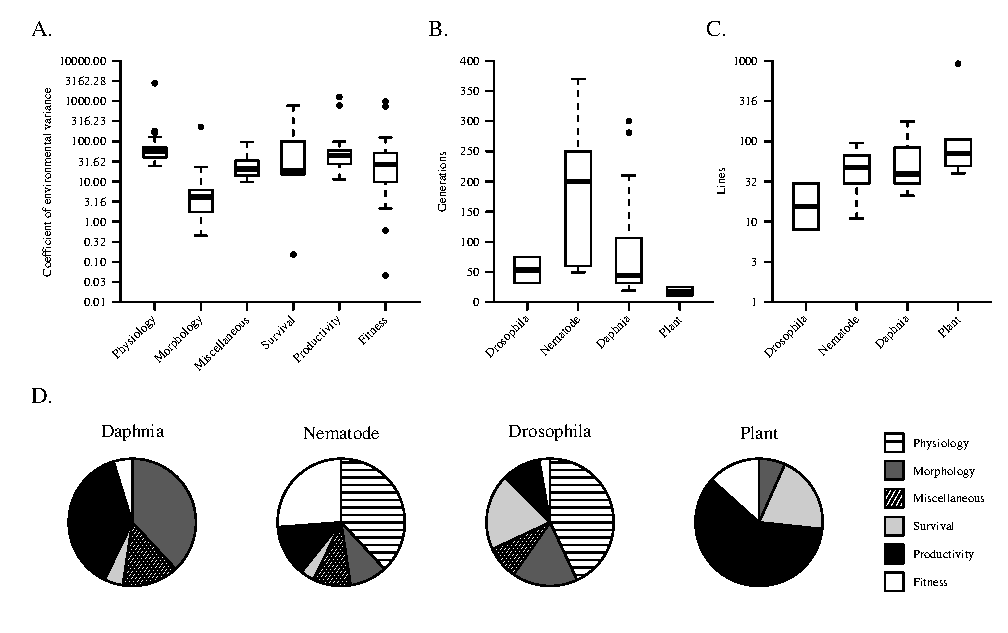
\includegraphics{Supp/Chp2_Meta/FigS2_11.02.22_45.eps}
    \caption[Variation of factors that may influence the magnitude of mutational variance estimates.]{\textbf{Variation of factors that may influence the magnitude of mutational variance estimates.} (A) $CV_E$ was calculated as$^1{:}~CV_E = \frac{\sqrt{V_E}}{\bar{X}}$ and log-transformed to improve resolution for plotting (NB:~the values are shown in the y-axis were back-transformed to the original $CV_E$ scale). $CV_E$ was plotted per trait category, which are defined in Methods and Table \ref{tab:TraitTypes}. (B) the number of generations and (C) the (log-transformed; but as in (A) the y-axis is shown on the original scale) number of lines of mutation accumulation experiments (studies) in different taxon categories. Taxon categories are defined in Methods. Box plots represent the median (bar), interquartile range (IQR,~box) and 3 IQR (whiskers) values of the published estimates, with more extreme values indicated by solid circles. (D) The distribution of estimate numbers across the different trait categories within each taxon group, where traits definitions as per Table \ref{tab:TraitTypes}. }
    \label{fig:S2metaPred}
    \small
    \vspace{0.5cm}
\noindent $^1$ Houle, D., B. Morikawa and M. Lynch, 1996 Comparing mutational variabilities. Genetics 143: 1467-1483
\normalsize
\end{figure}

\newpage
\FloatBarrier
\begin{figure}
    \centering
    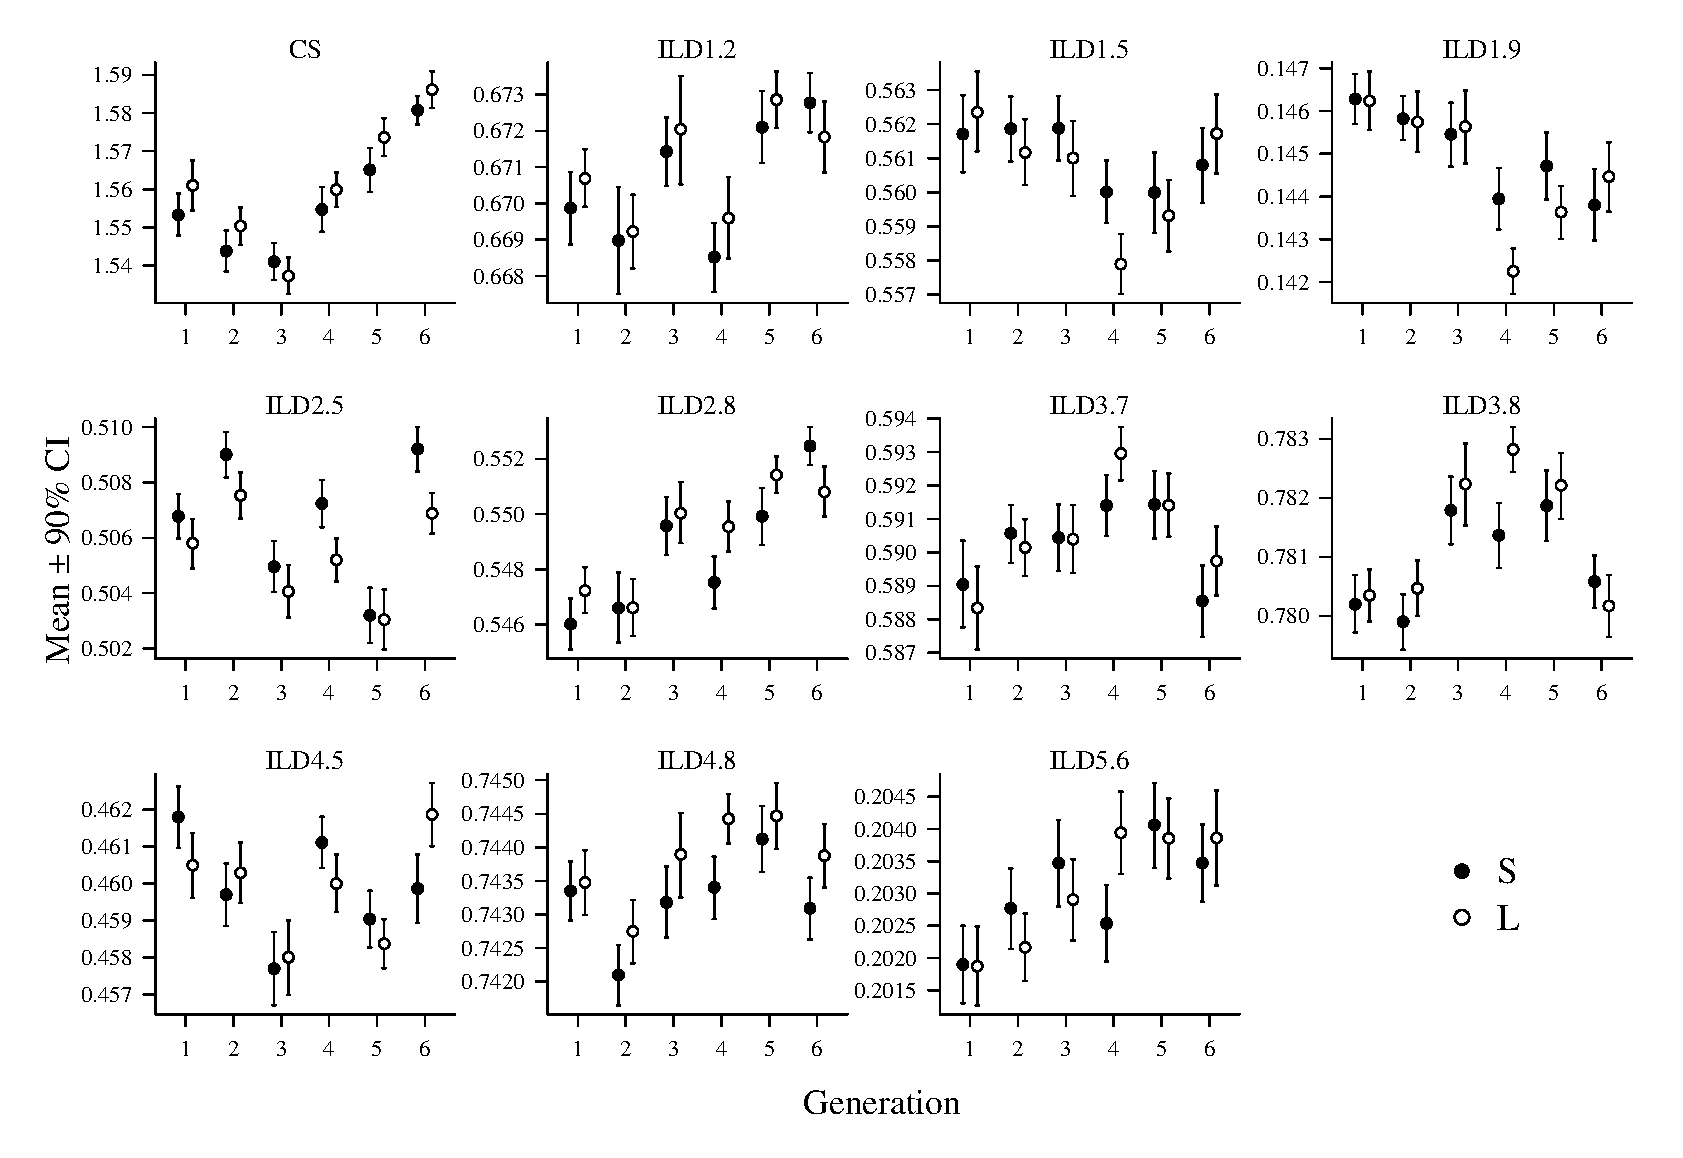
\includegraphics[width=0.95\textwidth]{Supp/Chp2_Meta/S3.Mean.eps}
    \caption[Variation in wing trait mean across six generations of an experiment in \textit{Drosophila serrata}.]{\textbf{Variation in wing trait mean across six generations of an experiment in \textit{Drosophila serrata}.} For each of the 11 wing traits (panels), the least-squares mean ($\pm$ 95\% CI) from model (\ref{eqn:metaUniVL}) is plotted for each generation for the Small (solid circle) and Large (open circles) population size treatments. Centroid size (CS) is measured in millimetres; the ten inter-landmark distances are in units of centroid size (multiplied by 100; see Figure \ref{fig:Fig2MetMRdsgn}B for trait definitions). Plotted estimates are reported in Table \ref{tab:S4RegCoef}.}
    \label{fig:S3TraitMean}
\end{figure}

% \newpage
% \FloatBarrier
\begin{figure}
    \centering
    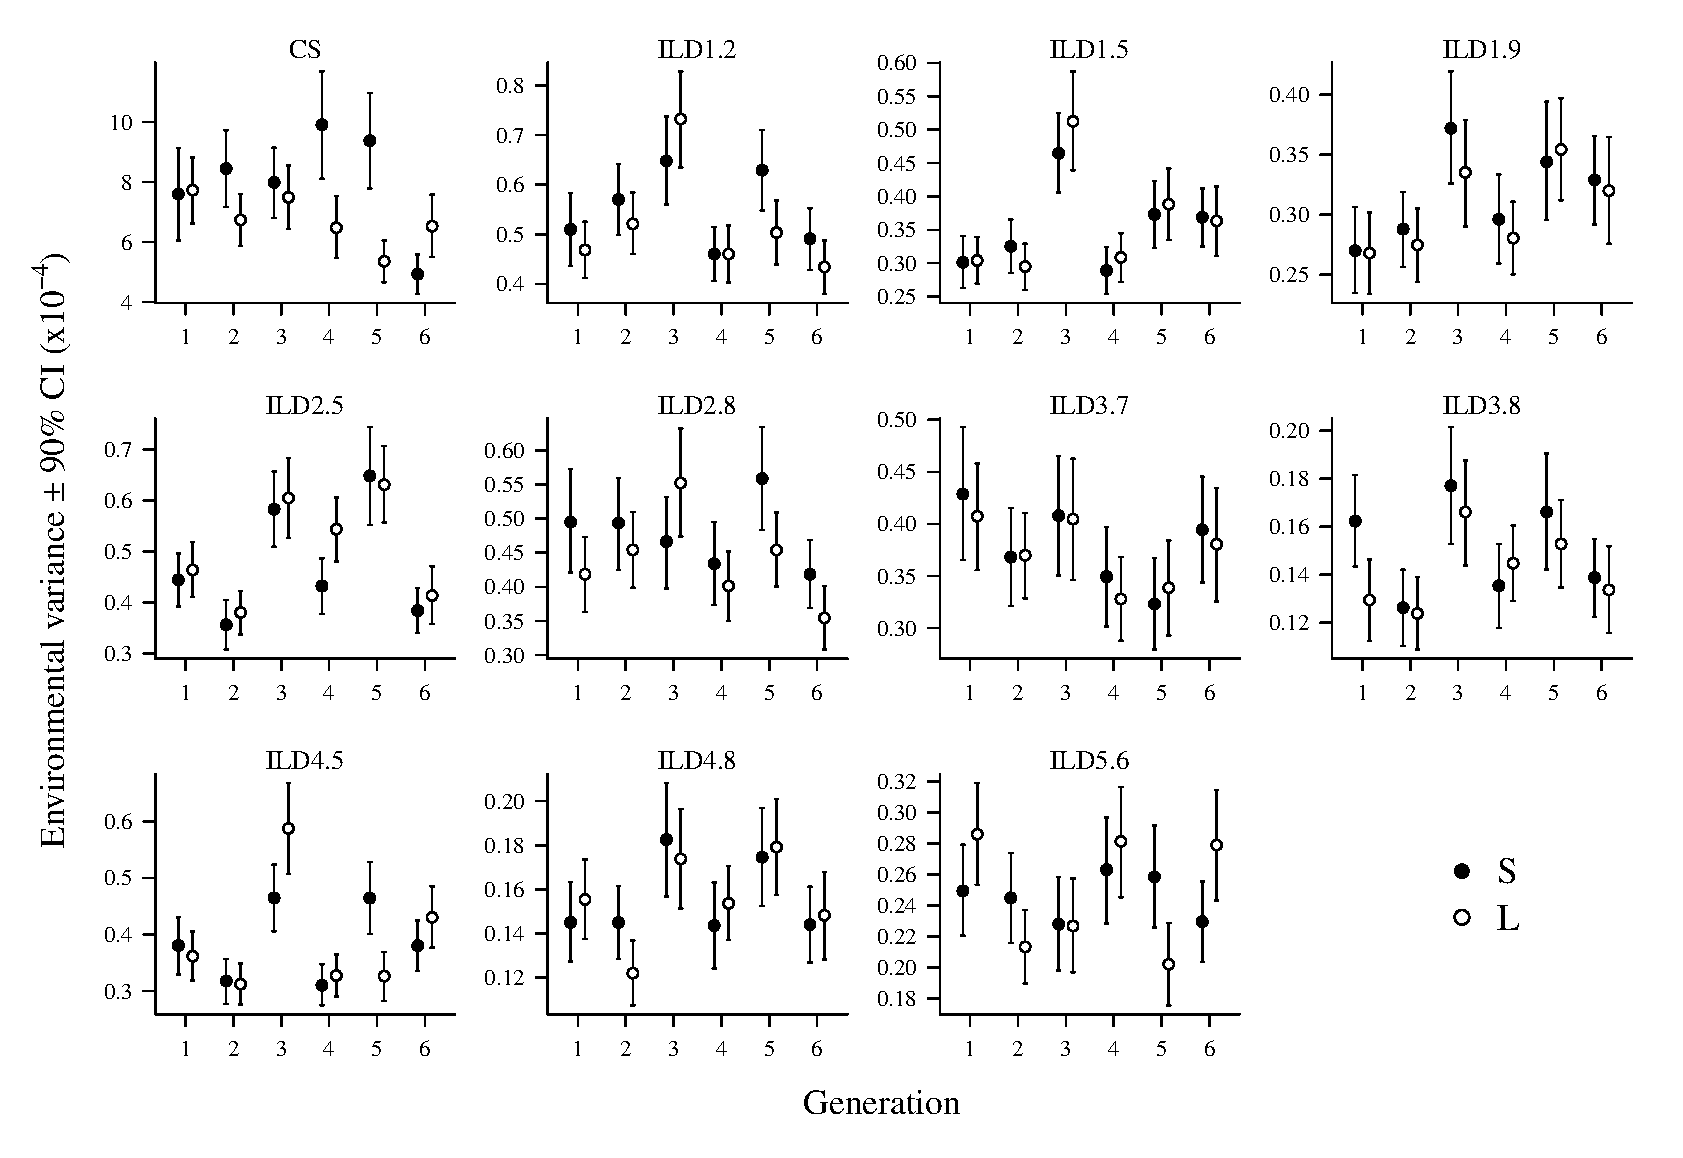
\includegraphics[width=0.95\textwidth]{Supp/Chp2_Meta/S4.Ve.eps}
    \caption[Variation in environmental variance across six generations of an experiment in \textit{Drosophila serrata}.]{\textbf{Variation in environmental variance across six generations of an experiment in \textit{Drosophila serrata}.} For each of the 11 wing traits (panels), $V_E$ ($\pm$ 95\% CI), estimated as the sum of among vial and residual variances from model (\ref{eqn:metaUniVL}), is plotted for each generation for the Small (solid~circle) and Large (open circles) population size treatments. Plotted estimates are reported in Table \ref{tab:S4RegCoef}.}
    \label{fig:S4Ve}
\end{figure}

% \newpage
% \FloatBarrier
\begin{figure}
    \centering
    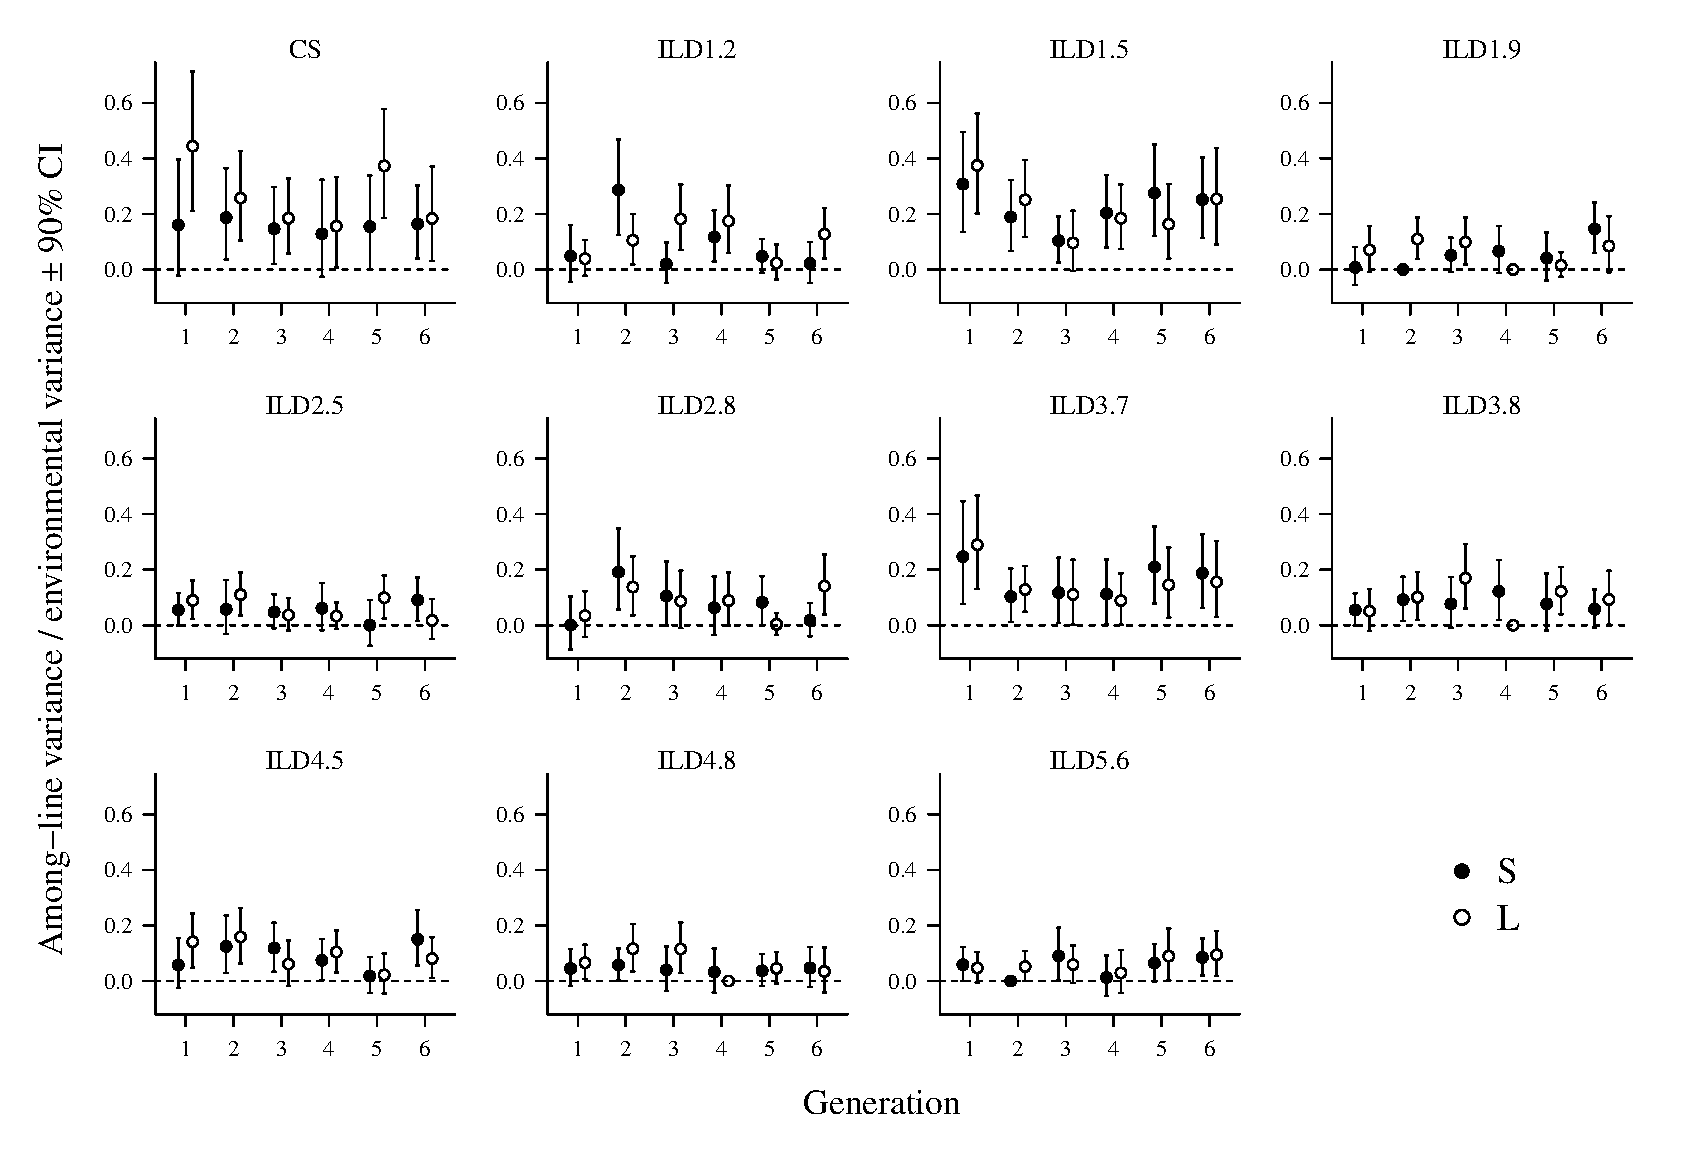
\includegraphics[width=0.95\textwidth]{Supp/Chp2_Meta/S5_VLVe.eps}
    \caption[Variance scaled estimates of among-line variance estimates in \textit{D. serrata}.]{\textbf{Variance scaled estimates of among-line variance estimates in \textit{D. serrata}.} Among-line variance estimates ($V_L$, Figure \ref{fig:Fig5VlBounce}) were placed on a heritability scale to account for the influence of trait variance on the magnitude of estimates, dividing $V_L$ by the corresponding estimate of environmental variance (summed among-vial and residual variance reported in Table \ref{tab:S4RegCoef}). Plotted are these variance-scaled REML estimates (90\% CI) for each trait (panel) (trait descriptions in Figure \ref{fig:Fig2MetMRdsgn}B) in each generation (x-axis) for each of the two population size treatments (Small:~solid circles; Large:~open circles). The dashed horizontal line indicates zero.}
    \label{fig:S5h2m}
\end{figure}

% \newpage
% \FloatBarrier
\begin{figure}
    \centering
    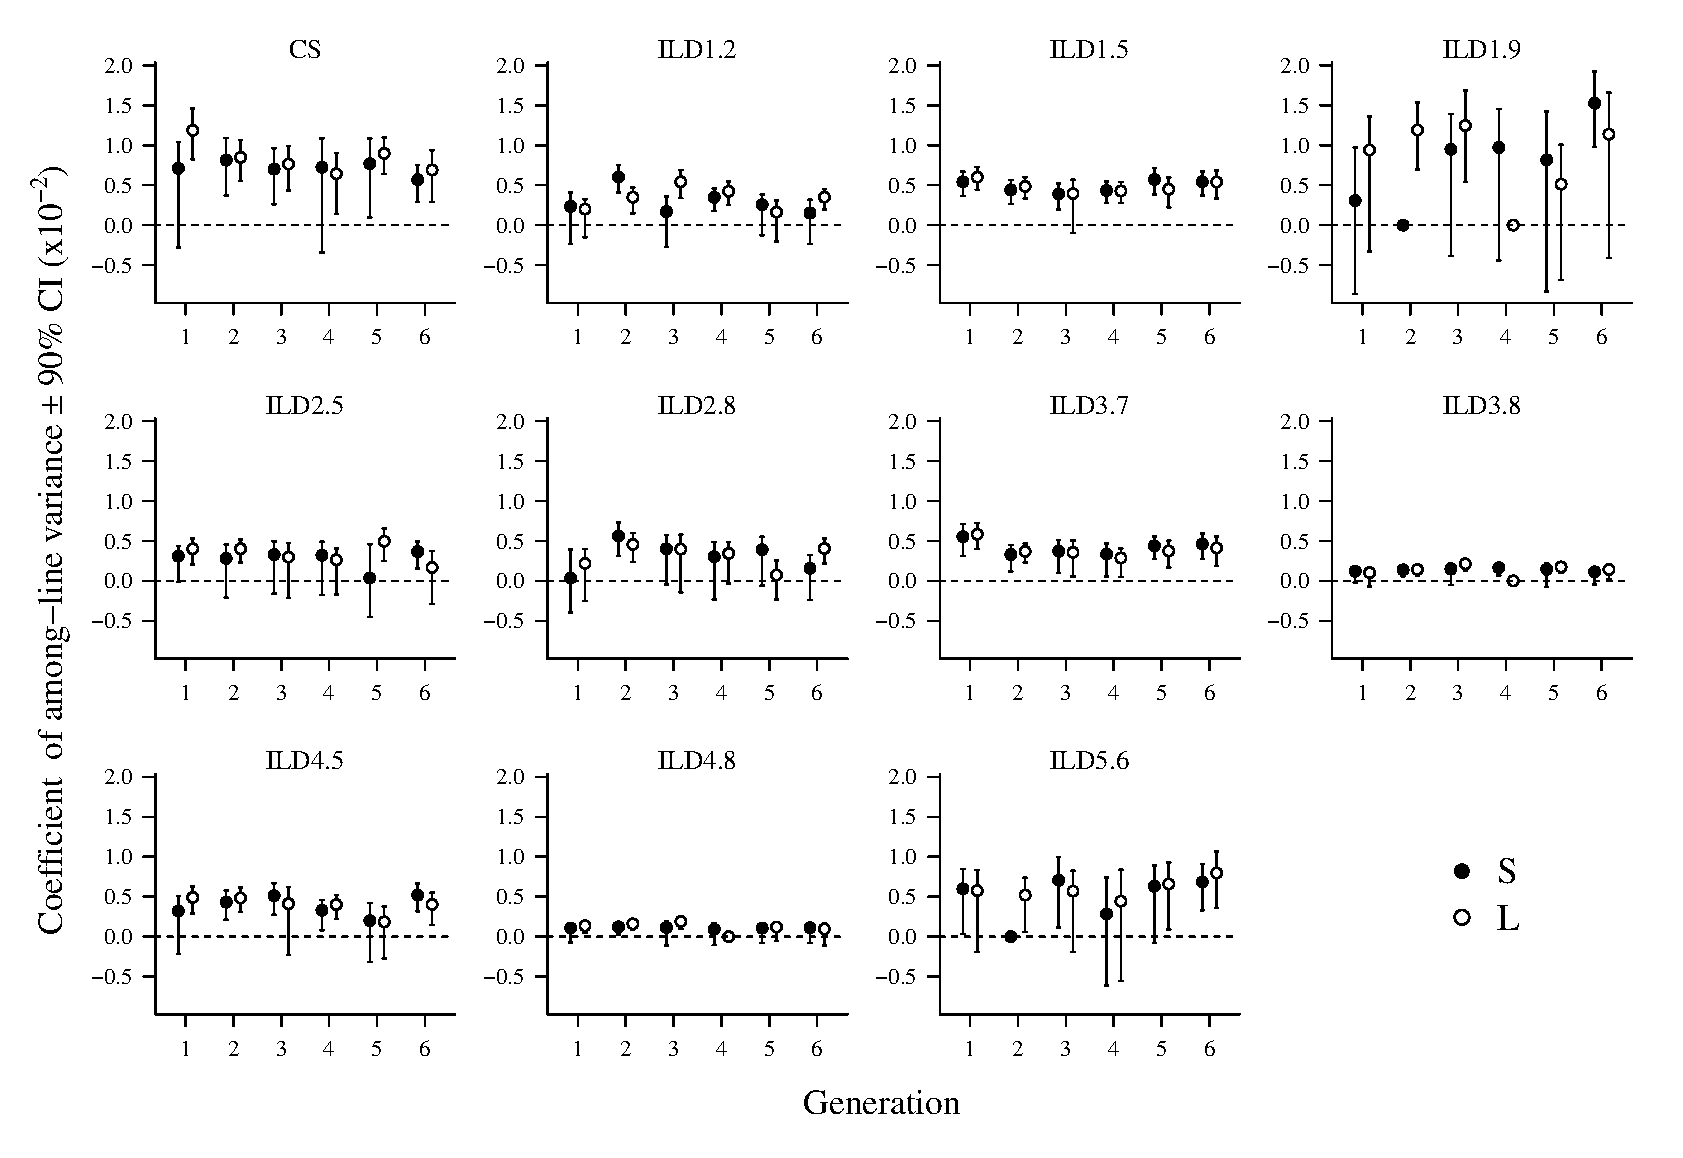
\includegraphics[width=0.95\textwidth]{Supp/Chp2_Meta/S6_CVM.eps}
    \caption[Mean-scaled estimates of among-line variance estimates in \textit{D. serrata}.]{\textbf{Mean-scaled estimates of among-line variance estimates in \textit{D. serrata}.} Among-line variance estimates ($V_L$, Figure \ref{fig:Fig5VlBounce}) were placed on a coefficient of variance scale to account for the influence of trait mean on magnitude of estimates, using the following formula: $100*\frac{\sqrt{V_L}}{\bar{X}}$ where $\bar{X}$ is the trait mean (Table \ref{tab:S4RegCoef}). Plotted are the REML point estimates (and 90\% CI) for each trait (panel) (see Figure \ref{fig:Fig2MetMRdsgn}B for trait descriptions) in each generation (x-axis) for each of the two population size treatments (Small: solid circles; Large: open circles). The dashed horizontal line indicates zero.}
    \label{fig:S6CVM}
\end{figure}

% \newpage
% \FloatBarrier
\begin{figure}
    \centering
    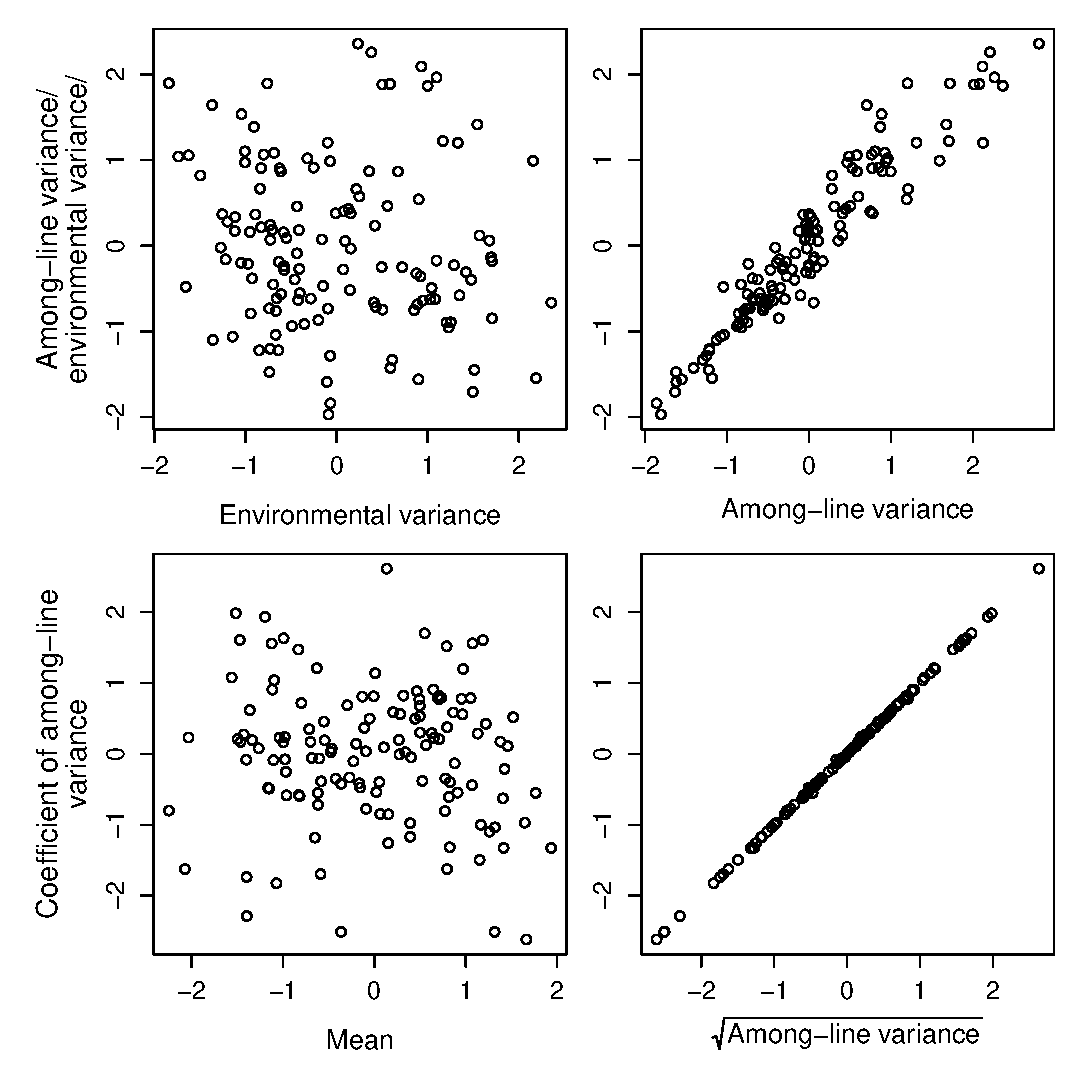
\includegraphics[width=0.75\textwidth]{Supp/Chp2_Meta/S7.Rel.Contribution.eps}
    \caption[The relative contributions of heterogeneity in the scaling parameter ($V_E$ or trait mean) and the among-line variance ($V_L$) to the variation observed in the variance-scaled or mean-scaled estimates of \textit{Drosophila serrata} among-line variance.]{\textbf{The relative contributions of heterogeneity in the scaling parameter ($V_E$ or trait mean; left panels) and the among-line variance ($V_L$; right panels) to the variation observed in the variance-scaled (top panels) or mean-scaled (bottom panel) estimates of \textit{Drosophila serrata} among-line variance.} All estimates are presented in Table \ref{tab:S4RegCoef}, $V_L$ is also presented in Figure \ref{fig:Fig5VlBounce}; $V_E$ and mean in Figures \ref{fig:S3TraitMean} and \ref{fig:S4Ve}, respectively; variance or mean scaled estimates of $V_L$ in Figures \ref{fig:S5h2m} and \ref{fig:S6CVM}, respectively. The 12 estimates for each of the 11 traits for each parameter ($V_L$, $V_E$, mean, variance-scaled and mean-scaled) were first placed on a standardised scale by centring on the mean of the 12 estimates, and dividing by the standard deviation of the 12 estimates (i.e., z-scores were calculated), and all 132 estimates (12 estimates per 11 traits) are plotted.}
    \label{fig:S7Heterogenity}
\end{figure}

% \newpage
% \FloatBarrier
\begin{figure}
    \centering
    \includegraphics[width=0.75\textwidth]{Supp/Chp2_Meta/S8.Est.CVs.eps}
    \vspace{-2cm}
    \caption[Variation in estimates of each genetic variation parameter in \textit{D. serrata}.]{\textbf{Variation in estimates of each genetic variation parameter in \textit{D. serrata}.} For each of these parameters, the 12 estimates per trait (Table \ref{tab:S4RegCoef}) were analysed to calculate the coefficient of variance, cv, across the 12 observations as: standard deviation / mean. Box plots represent the median (bar), interquartile range (IQR, box) and 3 IQR (whiskers) cv values for the 11 traits.}
    \label{fig:S8VarInCVs}
\end{figure}

